\documentclass[a4paper,11pt,notitlepage]{report}
% Henrik Kramselund  , February 2001
% hlk@security6.net,
% My standard packages
\usepackage{zencurity-exercises}

\begin{document}

\rm
\selectlanguage{english}
\newcommand{\subject}[1]{Communication and Network Security workshop}
\mytitle{Communication and Network Security}{exercises}

\setcounter{tocdepth}{0}

{\color{titlecolor}
\renewcommand{\baselinestretch}{0.3}\setlength{\parskip}{1mm}
\tableofcontents}
%\listoffigures - not used
%\listoftables - not used

\normal
\pagestyle{fancyplain}
\chapter*{\color{titlecolor}Preface}
\markboth{Preface}{}

This material was originally prepared for use in a course \emph{Communication and Network Security } and was prepared by
Henrik Kramselund  , \link{http://www.zencurity.com} .
It describes the networking setup and
applications for trainings and workshops where hands-on exercises are needed.

Further a presentation is used which is available as PDF from kramse@Github\\
Look for \jobname\ in the repo security-courses.

These exercises are expected to be performed in a training setting with network connected systems. The exercises use a number of tools which can be copied and reused after training. A lot is described about setting up your workstation in the repo

\link{https://github.com/kramse/kramse-labs}

Dont be scared away by the many exercises, you can pick a few and have fun with those and ignore the rest. If you one day need to research network security the others may come in handy \smiley

The exercise list includes my recommended tools I use myself and for teaching.

\section*{\color{titlecolor}Prerequisites}

This material expect that participants have a working knowledge of
TCP/IP from a user perspective. Basic concepts such as web site addresses and email should be known as well as IP-addresses and common protocols like DHCP.


\vskip 1cm
Have fun and learn



\begin{figure}[H]
\label{fig:osi}
\begin{center}
\colorbox{white}{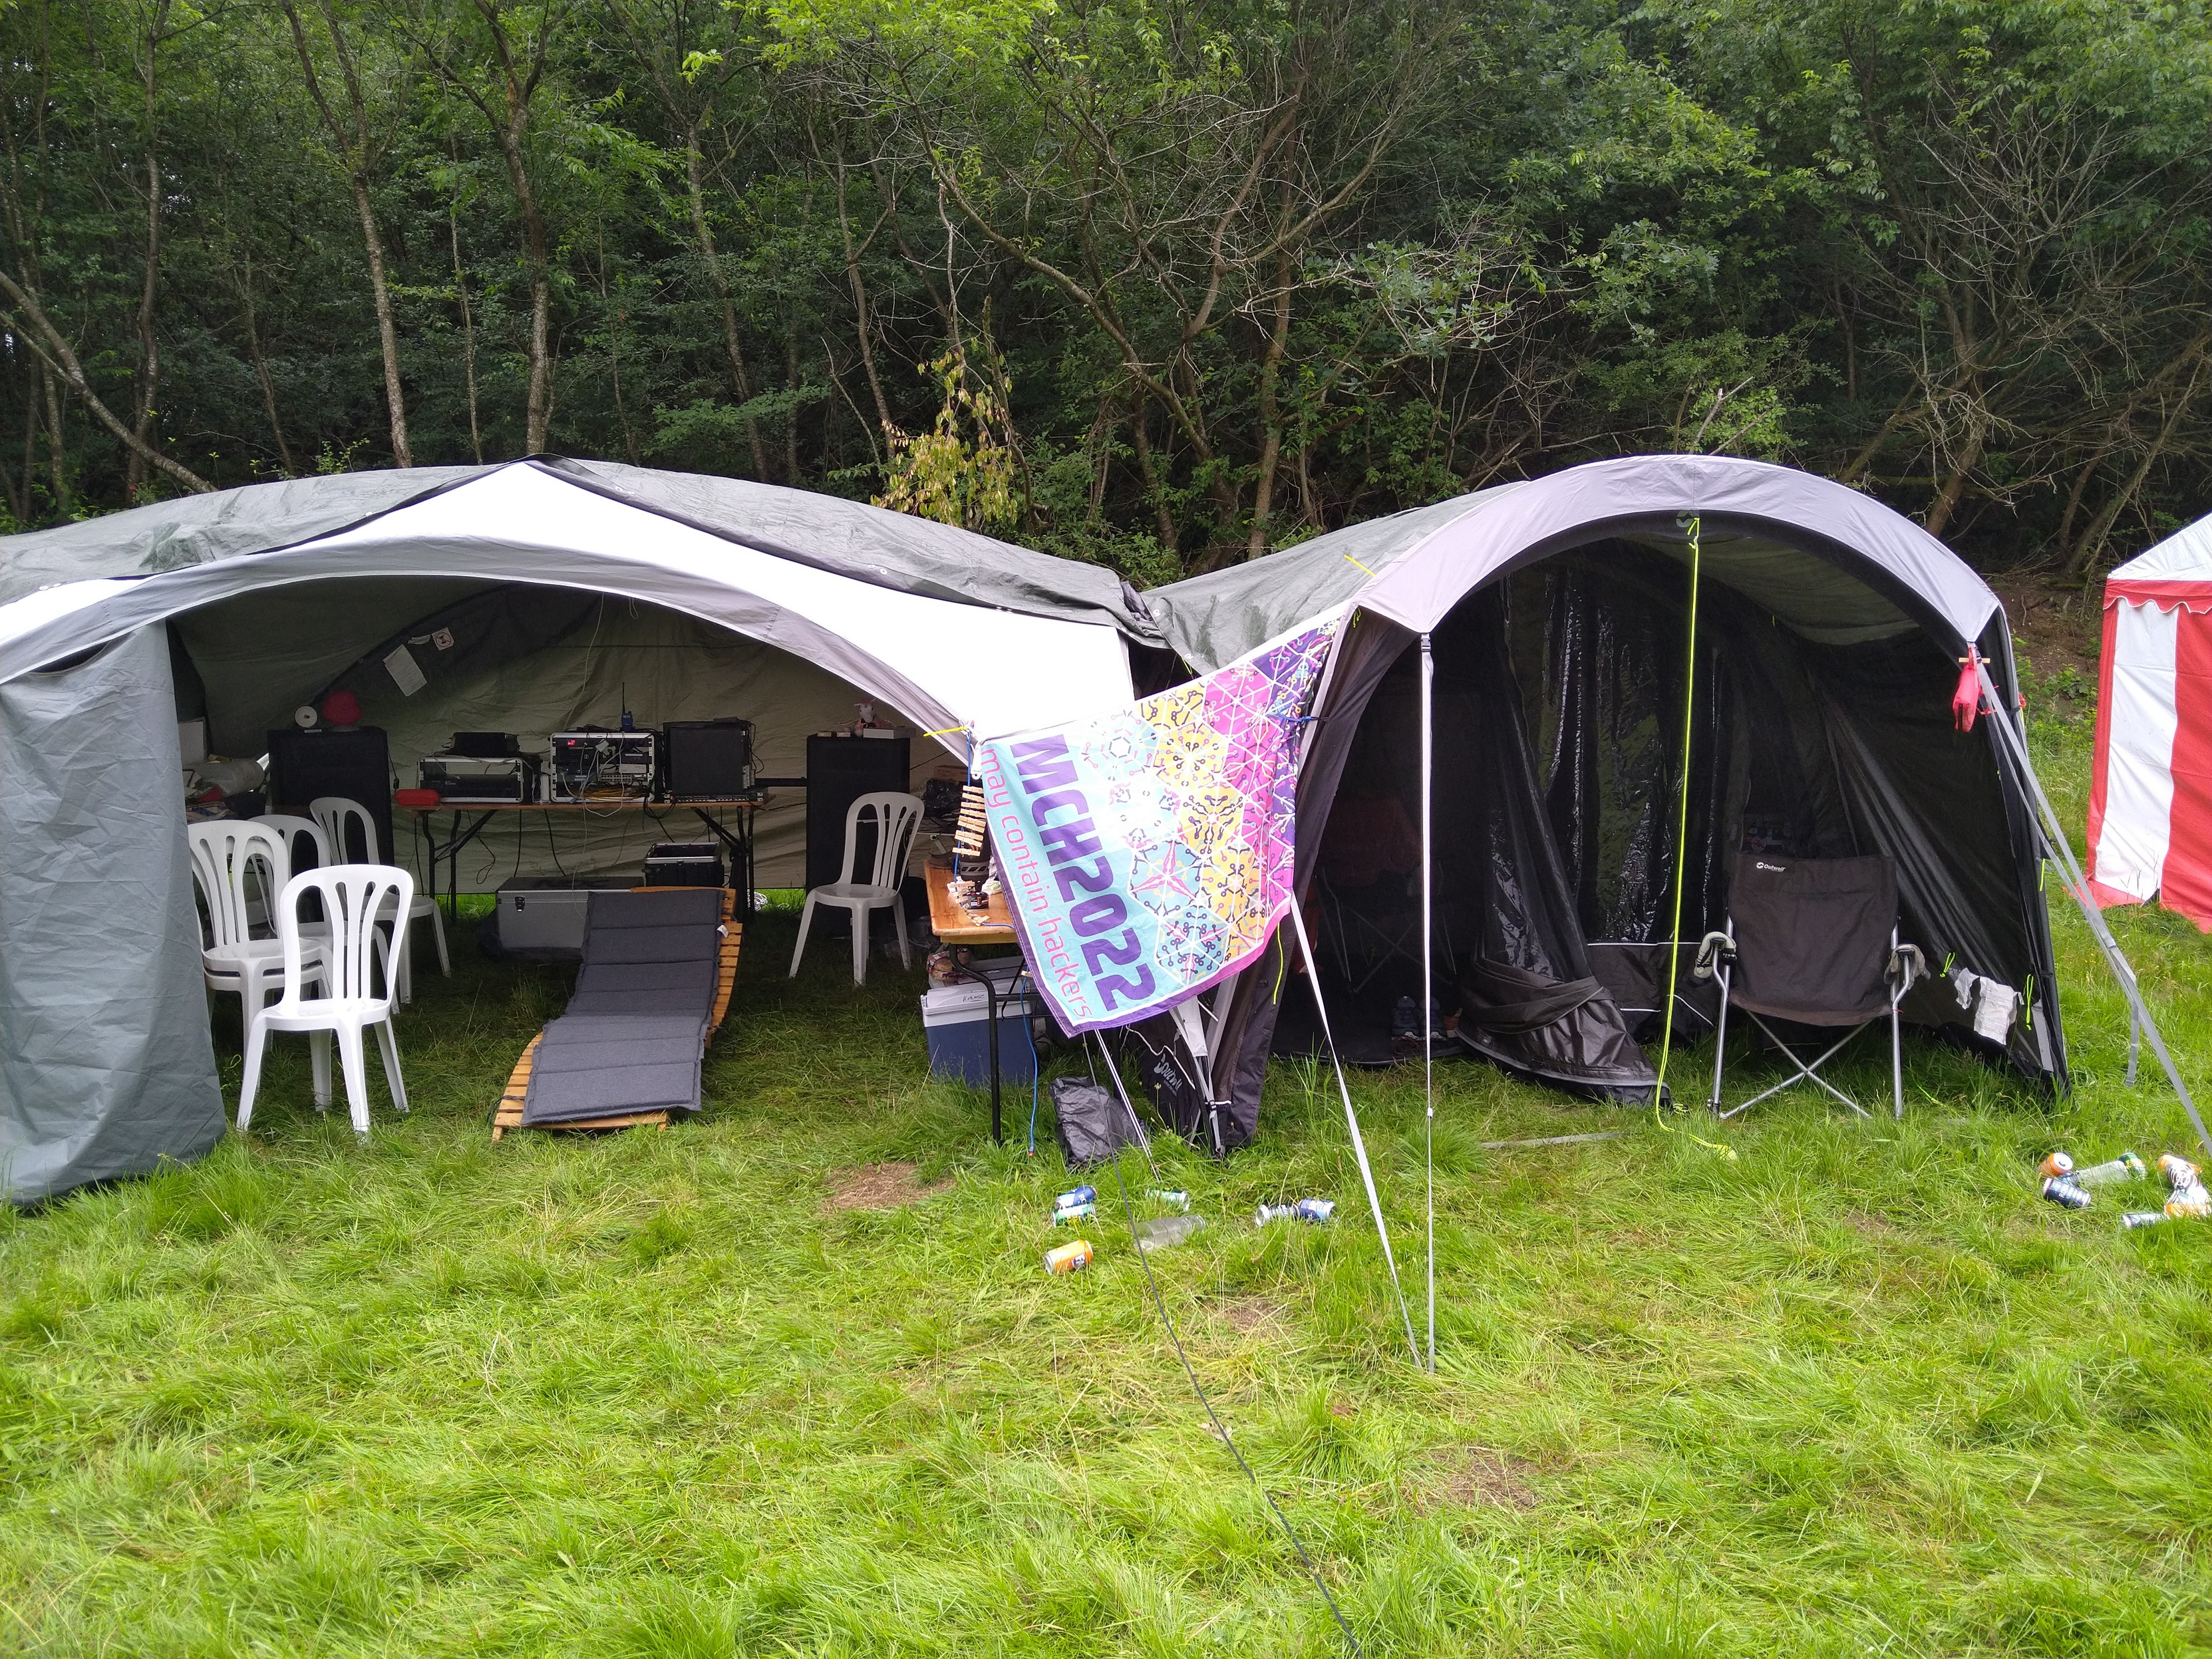
\includegraphics[width=10cm]{images/bornhack-camp-2024.jpg}}
\end{center}
\caption{The NWWC village at BornHack 2024}
\end{figure}


\eject

% =================== body of the document ===============
% Arabic page numbers
\pagenumbering{arabic}
\rhead{\fancyplain{}{\bf \chaptername\ \thechapter}}

% Main chapters
%---------------------------------------------------------------------
% gennemgang af emnet
% check questions


\chapter*{\color{titlecolor}Introduction to networking}
%\markboth{Introduktion til netværk}{}
\label{chap:intro}

\section*{\color{titlecolor}IP - Internet protocol suite}

It is extremely important to have a working knowledge about IP to implement
secure and robust infrastructures. Knowing about the alternatives while doing
implementation will allow the selection of the best features.

\section*{\color{titlecolor}ISO/OSI reference model}
A very famous model used for describing networking is the ISO/OSI model
of networking which describes layering of network protocols in stacks.

This model divides the problem of communicating into layers which can
then solve the problem as smaller individual problems and the solution
later combined to provide networking.

Having layering has proven also in real life to be helpful, for instance
replacing older hardware technologies with new and more efficient technologies
without changing the upper layers.

In the picture the OSI reference model is shown along side with
the Internet Protocol suite model which can also be considered to have different layers.


\begin{figure}[H]
\label{fig:osi}
\begin{center}
\colorbox{white}{\includegraphics[width=8cm,angle=90]{images/compare-osi-ip.pdf}}
\end{center}
\caption{OSI og Internet Protocol suite}
\end{figure}


\chapter*{\color{titlecolor}Exercise content}
\markboth{Exercise content}{}

Most exercises follow the same procedure and has the following content:
\begin{itemize}
\item {\bf Objective:} What is the exercise about, the objective
\item {\bf Purpose:} What is to be the expected outcome and goal of doing this exercise
\item {\bf Suggested method:} suggest a way to get started
\item {\bf Hints:} one or more hints and tips or even description how to
do the actual exercises
\item {\bf Solution:} one possible solution is specified
\item {\bf Discussion:} Further things to note about the exercises, things to remember and discuss
\end{itemize}

Please note that the method and contents are similar to real life scenarios and does not detail every step of doing the exercises. Entering commands directly from a book only teaches typing, while the exercises are designed to help you become able to learn and actually research solutions.



\chapter{\faInfoCircle\ Download Debian Administrator’s Handbook (DEB) Book 10 min}
\label{ex:sw-downloadDEB}

\hlkimage{3cm}{book-debian-administrators-handbook.jpg}


{\bf Objective:}\\
We need a Linux for running some tools during the course. I have chosen Debian Linux as this is open source, and the developers have released a whole book about running it.

This book is named
\emph{The Debian Administrator’s Handbook},  - shortened DEB

{\bf Purpose:}\\
Debian Linux is a mature Unix with great documentation. Kali Linux is based on Debian, so buy learning Debian you can make infrastructure using Debian Linux, and test security using Kali Linux -- and the administration will be the same commands.

in a few moments, so better have the instructions ready.

{\bf Suggested method:}\\
Create folders for educational materials. Go to download from the link \url{https://debian-handbook.info/}
Read and follow the instructions for downloading the book.

{\bf Solution:}\\
When you have a directory structure for download for this course, and the book DEB in PDF you are done.

{\bf Discussion:}\\
Linux is free and everywhere. The tools we will run in this course are made for Unix, so they run great on Linux.

Debian Linux is a free operating system platform.

The book DEB is free, but you can buy/donate to Debian, and I recommend it.


\chapter{\faExclamationTriangle\ Check your Kali VM, run Kali Linux 30 min}
\label{ex:basicKaliVM}

\hlkimage{10cm}{kali-linux.png}

{\bf Objective:}\\
Make sure your virtual machine is in working order.

If you have a Kali Linux for running tools most are preinstalled or can be installed using \verb+apt install+

{\bf Purpose:}\\
A Linux virtual machine will make it easy to sniff network traffic, has a lot of diagnostic tools like traceroute, ping, and can easily run more advanced ones like Nmap, Nping, Wireshark etc.

{\bf Suggested method:}\\
Go to \link{https://github.com/kramse/kramse-labs/}

Read the instructions for the setup of a Kali VM.

{\bf Hints:}\\
If you allocate enough memory and disk you wont have problems.

{\bf Solution:}\\
When you have a updated virtualisation software and Kali Linux, then we are good.

{\bf Discussion:}\\
Linux is free and everywhere. The tools we will run in this course are made for Unix, so they run great on Linux.

Kali Linux includes many hacker tools and should be known by anyone working in infosec.

\chapter{\faInfoCircle\ Check your Debian VM 10 min}
\label{ex:sw-basicDebianVM}

\hlkimage{7cm}{debian-xfce.png}

{\bf Objective:}\\
Make sure your virtual machine is in working order.

You dont need both a Debian Linux and Kali for running tools in this booklet, but some are better suited for either, so you can choose to install both.

{\bf Purpose:}\\
If your VM is not installed and updated we will run into trouble later.

{\bf Suggested method:}\\
Go to \link{https://github.com/kramse/kramse-labs/}

Read the instructions for the setup of a Debian VM.

{\Large \bf This is a bonus exercise - only one Debian is needed per team.}

{\bf Hints:}\\
If you allocate enough memory and disk you wont have problems.

{\bf I suggest 50G disk, 2CPU cores and 6Gb memory for this course, if you have this.}

{\bf Solution:}\\
When you have a updated virtualisation software and a running VM, then we are good.

{\bf Discussion:}\\
Linux is free and everywhere. The tools we will run in this course are made for Unix, so they run great on Linux.

Debian Linux allows us to run Ansible and provision a whole SIEM in very few minutes.




\chapter{\faExclamationTriangle\ Configure Sudo}
\label{ex:}

{\bf Objective:}\\
Learn how to configure the tool Sudo to allow administrative commands.

{\bf Purpose:}\\
Sudo is the most common method for switching from a normal user to root which is the administrative user for Unix. This command allows you to use your own password and execute highly privileged commands easily.

{\bf Suggested method:}\\
Not in sudoers file, cannot run sudo command

This can be fixed quite easily.

If you use the su command first, to switch user to root and run the visudo command:
\begin{alltt}
hlk@debian01:~$ su -
// enter password
# visudo
\end{alltt}
You will get an editor, where you enter below the root line, your username and a similar line:
\begin{alltt}
# User privilege specification
root ALL = (ALL:ALL) ALL
hlk ALL = (ALL:ALL) NOPASSWD: ALL
\end{alltt}

In the example my user is \verb+hlk+

Then use ctrl-x if using Nano, and exit the editor - saving this configuration file.

{\bf Hints:}\\
Most books about Unix has a convention to use the dollar sign if you are logged in as a regular user and the hash tag sign when logged in as root.
\begin{alltt}
hlk@debian01:~$ echo "Hi I am just a regular user"

root@debian01:~# echo "this is a command being run by root"
\end{alltt}


{\bf Solution:}\\
When you can switch between your user and root you are done.

{\bf Discussion:}\\
Note sudo has had many security vulnerabilities, so you should keep your system up to date using apt regularly, read about updates in the DEB book.


\chapter{\faExclamationTriangle\ Enable firewall - 15min}
\label{ex:debian-firewall}

{\bf Objective:}\\
Turn on a firewall and configure a few simple rules.

{\bf Purpose:}\\
See how easy it is to restrict incoming connections to a server.


{\bf Suggested method:}\\
Install a utility for firewall configuration.

You should also perform Nmap port scan with the firewall enabled and disabled.

{\bf Hints:}\\
Using the ufw package it is very easy to configure the firewall on Linux.

Install and configuration can be done using these commands.
\begin{minted}[fontsize=\footnotesize]{shell}
root@debian01:~# apt install ufw
Reading package lists... Done
Building dependency tree
Reading state information... Done
The following NEW packages will be installed:
  ufw
0 upgraded, 1 newly installed, 0 to remove and 0 not upgraded.
Need to get 164 kB of archives.
After this operation, 848 kB of additional disk space will be used.
Get:1 http://mirrors.dotsrc.org/debian stretch/main amd64 ufw all 0.35-4 [164 kB]
Fetched 164 kB in 2s (60.2 kB/s)
...
root@debian01:~# ufw allow 22/tcp
Rules updated
Rules updated (v6)
root@debian01:~# ufw enable
Command may disrupt existing ssh connections. Proceed with operation (y|n)? y
Firewall is active and enabled on system startup
root@debian01:~# ufw status numbered
Status: active

     To                         Action      From
     --                         ------      ----
[ 1] 22/tcp                     ALLOW IN    Anywhere
[ 2] 22/tcp (v6)                ALLOW IN    Anywhere (v6)
\end{minted}

Also allow port 80/tcp and port 443/tcp - and install a web server. Recommend Nginx \verb+apt-get install nginx+

{\bf Solution:}\\
When firewall is enabled and you can still connect to Secure Shell (SSH) and web service, you are done.

{\bf Discussion:}\\
Further configuration would often require adding source prefixes which are allowed to connect to specific services. If this was a database server the database service should probably not be reachable from all of the Internet.

Web interfaces also exist, but are more suited for a centralized firewall.

Configuration of this firewall can be done using ansible, see the documentation and examples at \url{https://docs.ansible.com/ansible/latest/modules/ufw_module.html}

Should you have both a centralized firewall in front of servers, and local firewall on each server? Discuss within your team.



\chapter{\faExclamationTriangle\ Git tutorials - 15min}
\label{ex:git-tutorial}


\hlkimage{3cm}{git-logo.png}

{\bf Objective:}\\
Try the program Git locally on your workstation

{\bf Purpose:}\\
Running Git will allow you to clone repositories from others easily. This is a great way to get new software packages, and share your own.

Git is the name of the tool, and Github is a popular site for hosting git repositories.

{\bf Suggested method:}\\
Run the program from your Linux VM. You can also clone from your Windows or Mac OS X computer. Multiple graphical front-end programs exist too.

Most important are Git clone and pull:
\begin{alltt}\footnotesize
user@Projects:tt$ {\bf git clone https://github.com/kramse/kramse-labs.git}
Cloning into 'kramse-labs'...
remote: Enumerating objects: 283, done.
remote: Total 283 (delta 0), reused 0 (delta 0), pack-reused 283
Receiving objects: 100% (283/283), 215.04 KiB | 898.00 KiB/s, done.
Resolving deltas: 100% (145/145), done.

user@Projects:tt$ {\bf cd kramse-labs/}

user@Projects:kramse-labs$ {\bf ls}
LICENSE  README.md  core-net-lab  lab-network  suricatazeek  work-station
user@Projects:kramse-labs$ git pull
Already up to date.
\end{alltt}

{\bf Hints:}\\
Browse the Git tutorials on \link{https://git-scm.com/docs/gittutorial}\\
and \link{https://guides.github.com/activities/hello-world/}

We will not do the whole tutorials within 15 minutes, but get an idea of the command line, and see examples. Refer back to these tutorials when needed or do them at home.

Note: you don't need an account on Github to download/clone repositories, but having an acccount allows you to save repositories yourself and is recommended.

{\bf Solution:}\\
When you have tried the tool and seen the tutorials you are done.

{\bf Discussion:}\\
Before Git there has been a range of version control systems,\\
see \link{https://en.wikipedia.org/wiki/Version\_control} for more details.





\chapter{\faExclamationTriangle\ Wireshark and Tcpdump 15 min}
\label{ex:wireshark-install}

\hlkimage{10cm}{wireshark-http.png}


{\bf Objective:}\\
Try the program Wireshark locally your workstation, or tcpdump

You can run Wireshark on your host too, if you want.

{\bf Purpose:}\\
Installing Wireshark will allow you to analyse packets and protocols

Tcpdump is a feature included in many operating systems and devices to allow packet capture and saving network traffic into files.

{\bf Suggested method:}\\
Run Wireshark or tcpdump from your Kali Linux

The PPA book page 41 describes Your First Packet Capture.

{\bf Hints:}\\
PCAP is a packet capture library allowing you to read packets from the network.
Tcpdump uses libpcap library to read packet from the network cards and save them.
Wireshark is a graphical application to allow you to browse through traffic, packets and protocols.

Both tools are already on your Kali Linux, or do: \verb+apt-get install tcpdump wireshark+

{\bf Solution:}\\
When Wireshark is installed sniff some packets. We will be working with both live traffic and saved packets from files in this course.

If you want to capture packets as a non-root user on Debian, then use the command to add a Wireshark group:
\begin{alltt}
sudo dpkg-reconfigure wireshark-common
\end{alltt}

and add your user to this:
\begin{alltt}
sudo gpasswd -a $USER wireshark
\end{alltt}
Dont forget to logout/login to pick up this new group.

{\bf Discussion:}\\
Wireshark is just an example other packet analyzers exist, some commercial and some open source like Wireshark

We can download a lot of packet traces from around the internet, we might use examples from\\
\link{https://old.zeek.org/community/traces.html}

\chapter{\faExclamationTriangle\ Capturing TCP Session packets 10 min}
\label{ex:wireshark-capture}

\hlkimage{6cm}{tcp-three-way.pdf}


{\bf Objective:}\\
Sniff TCP packets and dissect them using Wireshark

{\bf Purpose:}\\
See real network traffic, also know that a lot of information is available and not encrypted.

Note the three way handshake between hosts running TCP. You can either use a browser or command line tools like cURL while capturing

\begin{alltt}
curl http://www.zencurity.com
\end{alltt}

{\bf Suggested method:}\\
Open Wireshark and start a capture\\
Then in another window execute the ping program while sniffing

or perform a Telnet connection while capturing data

{\bf Hints:}\\
When running on Linux the network cards are usually named eth0 for the first Ethernet and wlan0 for the first Wireless network card. In Windows the names of the network cards are long and if you cannot see which cards to use then try them one by one.

{\bf Solution:}\\
When you have collected some TCP sessions you are done.

{\bf Discussion:}
Is it ethical to collect packets from an open wireless network?

Also note the TTL values in packets from different operating systems

\chapter{\faExclamationTriangle\ Whois databases 15 min}
\label{ex:whois}

{\bf Objective:}\\
Learn to lookup data in the global Whois databases

{\bf Purpose:}\\
We often need to see where traffic is coming from, or who is responsible for the IP addresses sending attacks.

{\bf Suggested method:}\\
Use a built-in command line, like: \verb+host www.zencurity.dk+ to look up an IP address and then \verb+whois + with the IP address.

{\bf Hints:}\\
Another option is to use web sites for doing Whois lookups \link{https://apps.db.ripe.net/db-web-ui/\#/query} or their RIPEStat web site which can give even more information
\link{https://stat.ripe.net/}

{\bf Solution:}\\
When you can find our external address and look it up, you are done.

{\bf Discussion:}\\
Whois databases are global and used for multiple purposes, the ones run by the Regional Internet Registries ARIN, RIPE, AfriNIC, LACNIC og APNIC have information about IP addresses and AS numbers allocated.


\chapter{\faExclamationTriangle\ IP address research 30 min}
\label{ex:ip-address-research}

{\bf Objective:}\\
Work with IP addresses

{\bf Purpose:}\\
What is an IP address?

Investigate the following IP addresses
\begin{list2}
\item 192.168.1.1
\item 192.0.2.0/24
\item 172.25.0.1
\item 182.129.62.63
\item 185.129.62.63
\end{list2}

Write down everything you can about them!

{\bf Suggested method:}\\
Search for the addresses, look for web sites that may help.

{\bf Hints:}\\
Download the fun guide from Julia Evans (b0rk) \url{https://jvns.ca/networking-zine.pdf}

Pay attention to Notation Time page

Lookup \url{ripe.net} they may have a service called stats or stat -- something like that.

What is the Torproject? good, bad, neutral?

{\bf Solution:}\\
When you have found some information about each of the above, say 2-3 facts about each you are done.

{\bf Discussion:}\\
IP addresses are much more than an integer used for addressing system interfaces and routing packets.

We will later talk more about \emph{IP reputation}


\chapter{\faExclamationTriangle\ Using ping and traceroute 10 min}
\label{ex:ping}



{\bf Objective:}\\
Be able to do initial debugging of network problems using commands ping and traceroute

{\bf Purpose:}\\
Being able to verify connectivity is a basic skill.

{\bf Suggested method:}\\
Use \verb+ping+ and \verb+traceroute+ to test your network connection - can be done one Windows and UNIX.

{\bf Hints:}
\begin{alltt}\small
$ ping 10.0.42.1
PING 10.0.42.1 (10.0.42.1) 56(84) bytes of data.
64 bytes from 10.0.42.1: icmp_seq=1 ttl=62 time=1.02 ms
64 bytes from 10.0.42.1: icmp_seq=2 ttl=62 time=0.998 ms
^C
--- 10.0.42.1 ping statistics ---
2 packets transmitted, 2 received, 0% packet loss, time 1001ms
rtt min/avg/max/mdev = 0.998/1.012/1.027/0.034 ms
\end{alltt}

Dont forget that UNIX ping continues by default, press ctrl-c to break.

Do the same with traceroute.

{\bf Solution:}\\
Run both programs to local gateway and some internet address by your own choice.

{\bf Discussion:}\\
Note the tool is called tracert on Windows, shortened for some reason.

ICMP is the Internet Control Message Protocol, usually used for errors like host unreachable. The ECHO request ICMP message is the only ICMP message that generates another.

The traceroute programs send packets with low Time To Live (TTL) and receives ICMP messages, unless there is a problem or a firewall/filter. Also used for mapping networks.

{\bf \faInfoCircle\ }

Whats the difference between:
\begin{list2}
\item {\bfseries traceroute} and {\bfseries traceroute -I}
\item NB: traceroute -I is found on UNIX - traceroute using ICMP pakker
\item Windows tracert by default uses ICMP
\item Unix by default uses UDP, but can use ICMP instead.
\item Lots of traceroute-like programs exist for tracing with TCP or other protocols
\end{list2}


\chapter{\faExclamationTriangle\ DNS and Name Lookups 10 min}
\label{ex:basic-dns-lookup}



{\bf Objective:}\\
Be able to do DNS lookups from specific DNS server

{\bf Purpose:}\\
Try doing DNS lookup using different programs

{\bf Suggested method:}\\
Try the following programs:
\begin{itemize}
\item nslookup - UNIX and Windows, but not recommended\\
\verb+nslookup -q=txt -class=CHAOS version.bind. 0+
\item dig - syntax @server domain query-type query-class\\
\verb+dig @8.8.8.8 www.example.com+
\item host - syntaks host [-l] [-v] [-w] [-r] [-d] [-t querytype] [-a] host [server]\\
\verb+host www.example.com 8.8.8.8+
\end{itemize}

{\bf Hints:}\\
Dig is the one used by most DNS admins, I often prefer the host command for the short output.

{\bf Solution:}\\
Shown inline, above.

{\bf Discussion:}\\
The nslookup program does not use the same method for lookup as the standard lookup libraries, results may differ from what applications see.

What is a zone transfer, can you get one using the host command?

Explain forward and reverse DNS lookup.




\chapter{\faExclamationTriangle\ Nping check ports 10 min}
\label{ex:nping-tcp}
{\bf Objective:} \\
Show the use of Nping tool for checking ports through a network

{\bf Purpose:}\\
Nping can check if probes can reach through a network, reporting success of failure. Allows very specific packets to be sent. It is part of the Nmap package.

{\bf Suggested method:}\\
Run the command using a common port like Web HTTP:
\begin{alltt}\footnotesize
root@KaliVM:~# nping --tcp -p 80 www.zencurity.com

Starting Nping 0.7.70 ( https://nmap.org/nping ) at 2018-09-07 19:06 CEST
SENT (0.0300s) TCP 10.137.0.24:3805 > 185.129.60.130:80 S ttl=64 id=18933 iplen=40  seq=2984847972 win=1480
RCVD (0.0353s) TCP 185.129.60.130:80 > 10.137.0.24:3805 SA ttl=56 id=49674 iplen=44  seq=3654597698 win=16384 <mss 1460>
SENT (1.0305s) TCP 10.137.0.24:3805 > 185.129.60.130:80 S ttl=64 id=18933 iplen=40  seq=2984847972 win=1480
RCVD (1.0391s) TCP 185.129.60.130:80 > 10.137.0.24:3805 SA ttl=56 id=50237 iplen=44  seq=2347926491 win=16384 <mss 1460>
SENT (2.0325s) TCP 10.137.0.24:3805 > 185.129.60.130:80 S ttl=64 id=18933 iplen=40  seq=2984847972 win=1480
RCVD (2.0724s) TCP 185.129.60.130:80 > 10.137.0.24:3805 SA ttl=56 id=9842 iplen=44  seq=2355974413 win=16384 <mss 1460>
SENT (3.0340s) TCP 10.137.0.24:3805 > 185.129.60.130:80 S ttl=64 id=18933 iplen=40  seq=2984847972 win=1480
RCVD (3.0387s) TCP 185.129.60.130:80 > 10.137.0.24:3805 SA ttl=56 id=1836 iplen=44  seq=3230085295 win=16384 <mss 1460>
SENT (4.0362s) TCP 10.137.0.24:3805 > 185.129.60.130:80 S ttl=64 id=18933 iplen=40  seq=2984847972 win=1480
RCVD (4.0549s) TCP 185.129.60.130:80 > 10.137.0.24:3805 SA ttl=56 id=62226 iplen=44  seq=3033492220 win=16384 <mss 1460>

Max rtt: 40.044ms | Min rtt: 4.677ms | Avg rtt: 15.398ms
Raw packets sent: 5 (200B) | Rcvd: 5 (220B) | Lost: 0 (0.00%)
Nping done: 1 IP address pinged in 4.07 seconds
\end{alltt}

{\bf Hints:} \\
A lot of options are similar to Nmap

{\bf Solution:}\\
When you have tried it towards an open port, a closed port and an IP/port that is filtered you are done.

{\bf Discussion:}\\
A colleague of ours had problems sending specific IPsec packets through a provider. Using a tool like Nping it is possible to show what happens, or where things are blocked.

\eject
Things like changing the TTL may provoke ICMP messages, like this:
\begin{alltt}\footnotesize
root@KaliVM:~# nping --tcp -p 80 --ttl 3 www.zencurity.com

Starting Nping 0.7.70 ( https://nmap.org/nping ) at 2018-09-07 19:08 CEST
SENT (0.0303s) TCP 10.137.0.24:37244 > 185.129.60.130:80 S ttl=3 id=60780 iplen=40  seq=1997801125 win=1480
RCVD (0.0331s) ICMP [10.50.43.225 > 10.137.0.24 TTL=0 during transit (type=11/code=0) ] IP [ttl=62 id=28456 iplen=72 ]
SENT (1.0314s) TCP 10.137.0.24:37244 > 185.129.60.130:80 S ttl=3 id=60780 iplen=40  seq=1997801125 win=1480
RCVD (1.0337s) ICMP [10.50.43.225 > 10.137.0.24 TTL=0 during transit (type=11/code=0) ] IP [ttl=62 id=28550 iplen=72 ]
SENT (2.0330s) TCP 10.137.0.24:37244 > 185.129.60.130:80 S ttl=3 id=60780 iplen=40  seq=1997801125 win=1480
RCVD (2.0364s) ICMP [10.50.43.225 > 10.137.0.24 TTL=0 during transit (type=11/code=0) ] IP [ttl=62 id=28589 iplen=72 ]
SENT (3.0346s) TCP 10.137.0.24:37244 > 185.129.60.130:80 S ttl=3 id=60780 iplen=40  seq=1997801125 win=1480
RCVD (3.0733s) ICMP [10.50.43.225 > 10.137.0.24 TTL=0 during transit (type=11/code=0) ] IP [ttl=62 id=29403 iplen=72 ]
SENT (4.0366s) TCP 10.137.0.24:37244 > 185.129.60.130:80 S ttl=3 id=60780 iplen=40  seq=1997801125 win=1480
RCVD (4.0558s) ICMP [10.50.43.225 > 10.137.0.24 TTL=0 during transit (type=11/code=0) ] IP [ttl=62 id=30235 iplen=72 ]

Max rtt: 38.574ms | Min rtt: 2.248ms | Avg rtt: 13.143ms
Raw packets sent: 5 (200B) | Rcvd: 5 (360B) | Lost: 0 (0.00%)
Nping done: 1 IP address pinged in 4.07 seconds
\end{alltt}


\chapter{\faInfoCircle\ Try pcap-diff 15 min}
\label{ex:pcap-diff}

{\bf Objective:}\\
Try both getting an utility tool from Github and running an actual useful tool for comparing packet captures.

{\bf Purpose:}\\
Being able to get tools and scripts from Github makes you more effective.

The tool we need today is \link{https://github.com/isginf/pcap-diff}

{\bf Suggested method:}\\
Git clone the repository, follow instructions for running a packet diff.

Try saving a few packets in a packet capture, then using tcpdump read and write a subset - so you end up with two packet captures:
\begin{alltt}\footnotesize
sudo tcpdump -w icmp-dump.cap
// run ping in another window, which probably creates ARP packets
// Check using tcpdump
sudo tcpdump -r icmp-dump.cap arp
reading from file icmp-dump.cap, link-type EN10MB (Ethernet)
10:06:18.077055 ARP, Request who-has 10.137.0.22 tell 10.137.0.6, length 28
10:06:18.077064 ARP, Reply 10.137.0.22 is-at 00:16:3e:5e:6c:00 (oui Unknown), length 28
10:06:24.776987 ARP, Request who-has 10.137.0.6 tell 10.137.0.22, length 28
10:06:24.777107 ARP, Reply 10.137.0.6 is-at fe:ff:ff:ff:ff:ff (oui Unknown), length 28
// Write the dump - but without the ARP packets:
sudo tcpdump -r icmp-dump.cap -w icmp-dump-no-arp.cap not arp
\end{alltt}

With these pcaps you should be able to do:
\begin{alltt}\footnotesize
sudo pip install scapy
git clone https://github.com/isginf/pcap-diff.git
cd pcap-diff/

$ python pcap_diff.py -i ../icmp-dump.cap -i ../icmp-dump-no-arp.cap -o diff.cap
Reading file ../icmp-dump.cap:
Found 23 packets

Reading file ../icmp-dump-no-arp.cap:
Found 19 packets

Diffing packets:

Found 2 different packets

Writing diff.cap
// Try reading the output packet diff:

$ sudo tcpdump -r diff.cap
reading from file diff.cap, link-type EN10MB (Ethernet)
10:06:24.777107 ARP, Reply 10.137.0.6 is-at fe:ff:ff:ff:ff:ff (oui Unknown), length 28
10:06:24.776987 ARP, Request who-has 10.137.0.6 tell 10.137.0.22, length 28
\end{alltt}

Note: I ran these on a Debian, so I needed the sudo, if you run this on Kali there is no need to use sudo.

{\bf Hints:}\\
Git is one of the most popular software development tools, and Github is a very popular site for sharing open source tools.

{\bf Solution:}\\
When you or your team mate has a running pcap-diff then you are done

{\bf Discussion:}\\
I often find that 90\% of my tasks can be done using existing open source tools.

\chapter{\faExclamationTriangle\ Discover active systems ping sweep 10 min}
\label{ex:nmap-pingsweep}
\hlkimage{5cm}{nmap-zenmap.png}

{\bf Objective:}\\
Use nmap to discover active systems

{\bf Purpose:}\\
Know how to use nmap to scan networks for active systems.

{\bf Suggested method:}\\

Due to python version 2 being deprecated there are some missing files for running the tool Zenmap. This can be fixed by using the Kali Kaboxer \verb+apt install zenmap-kbx+

Process is described in various posts around the internet. \link{https://www.kali.org/blog/introducing-kaboxer/}

The command to run Zenmap becomes: \verb+zenmap-kbx+\\
As always try typing zen and press TAB twice, will show all commands starting with these letters.

Try different scans,
\begin{itemize}
\item Ping sweep to find active systems
\item Port sweeps to find active systems with specific ports
\end{itemize}

{\bf Hints:} \\
Try nmap in sweep mode - and you may run this from Zenmap

{\bf Solution:}\\
Use the command below as examples:
\begin{itemize}
\item Ping sweep \verb+nmap -sP 10.0.45.*+
\item Port sweeps \verb+nmap -p 80 10.0.45.*+
\end{itemize}

{\bf Discussion:}\\
Quick scans quickly reveal interesting hosts, ports and services

Also now make sure you understand difference between single host scan
10.0.45.123/32, a whole subnet /24 ~250 hosts 10.0.45.0/24 and other more advanced targeteting like 10.0.45.0/25 and 10.0.45.1-10


\chapter{\faExclamationTriangle\ Execute nmap TCP and UDP port scan 20 min}
\label{ex:nmap-synscan}


{\bf Objective:} \\
Use nmap to discover important open ports on active systems

{\bf Purpose:}\\
Finding open ports will allow you to find vulnerabilities on these ports.

{\bf Suggested method:}\\
Use \verb+nmap -p 1-1024 server+ to scan the first 1024 TCP
ports and use Nmap without ports. What is scanned then?

Try to use \verb+nmap -sU+ to scan using UDP ports, not really possible if a firewall is in place.

If a firewall blocks ICMP you might need to add \verb+-Pn+ to make nmap scan even if there are no Ping responses

{\bf Hints:} \\
Sample command: \verb+nmap -Pn -sU -p1-1024 server+ UDP port scanning
1024 ports without doing a Ping first

{\bf Solution:}\\
Discover some active systems and most interesting ports, which are 1-1024 and the built-in list of popular ports.

{\bf Discussion:}\\
There is a lot of documentation about the nmap portscanner, even a book by the author
of nmap. Make sure to visit \link{http://www.nmap.org}

TCP and UDP is very different when scanning. TCP is connection/flow oriented and requires a handshake which is very easy to identify. UDP does not have a handshake and most applications will not respond to probes from nmap. If there is no firewall the operating system will respond to UDP probes on closed ports - and the ones that do not respond must be open.

When doing UDP scan on the internet you will almost never get a response, so you cannot tell open (not responding services) from blocked ports (firewall drop packets). Instead try using specific service programs for the services, sample program could be \verb+nsping+ which sends DNS packets, and will often get a response from a DNS server running on UDP port 53.

\chapter{\faExclamationTriangle\ Perform nmap OS detection 10 min}
\label{ex:nmap-os}

{\bf Objective:} \\
Use nmap OS detection and see if you can guess the brand of devices on the network

{\bf Purpose:}\\
Getting the operating system of a system will allow you to focus your next attacks.

{\bf Suggested method:}\\
Look at the list of active systems, or do a ping sweep.

Then add the OS detection using the option \verb+-O+



{\bf Hints:} \\
The nmap tool can send a lot of packets that will get different responses, depending on the operating system. TCP/IP is implemented using various constants chosen by the implementors, they have chosen different standard packet TTL etc.

{\bf Solution:}\\
Use a command like \verb+nmap -O -p1-100 10.0.45.45+ or  \verb+nmap -A -p1-100 10.0.45.45+


{\bf Discussion:}\\
Nmap OS detection is not a full proof way of knowing the actual operating system, but in most cases in can detect the family and in some cases it can identify the exact patch level of the system.

Better to use \verb+-A+ all the time, includes even more scripts and advanced stuff
You can also save prefixes to scan in a text file, I usually name it \verb+targets+

I also recommend adding \verb+-oA+ for writing output files. So a regular Nmap command might be:
\verb+nmap -p 1-65535 -A -oA full-tcp-scan -iL targets+


\chapter{\faInfoCircle\ EtherApe 10 min}
\label{ex:etherape}

\hlkimage{7cm}{etherape-2018.png}

\begin{quote}
EtherApe is a graphical network monitor for Unix modeled after etherman. Featuring link layer, IP and TCP modes, it displays network activity graphically. Hosts and links change in size with traffic. Color coded protocols display.
Node statistics can be exported.
\end{quote}

{\bf Objective:}\\
Use a tool to see more about network traffic, whats going on in a network.

{\bf Purpose:}\\
Get to know the concept of a node by seeing nodes communicate in a graphical environment.

{\bf Suggested method:}\\
Use the tool from Kali

The main page for the tool is:
\link{https://etherape.sourceforge.io/}

{\bf Hints:}\\
Your built-in Wi-Fi network card may not be the best for sniffing in promiscious and monitor mode.

Put your network card for the virtual system into bridging mode, and produce some data using Nmap ping scanning. Something like this for your local network \verb+nmap -sP 192.168.0.0/24+

{\bf Solution:}\\
When you have the tool running and showing data, you are done.

{\bf Discussion:}\\


\chapter{\faInfoCircle\ ARP spoofing and ettercap 20min}
\label{ex:arp-spoof-ettercap}


\hlkimage{7cm}{ettercap.png}

{\bf Objective:}\\
Use a tool to see more about network traffic, whats going on in a network.

{\bf Purpose:}\\
Start the tool, do a scan and start sniffing between your laptop and the router.

{\bf Suggested method:}
\begin{enumerate}
\item Start the tool using \verb+ettercap --gtk+ to get the graphical version.
\item Select menu Info, Help - and read about unified and bridged sniffing.
\item Start Unified sniffing from Sniff, Unified sniffing - select your network card.
\item Select Hosts - Scan
\end{enumerate}

You should be able to see some hosts. Then the next step would be to initiate attacks - which are menu-driven and easy to perform.

You might ruin the network temporarily for others when playing with this, so be cautious.

{\bf Hints:}\\
We might be messing to much with the traffic, so attacks wont succeed. Some coordination is needed.

{\bf Solution:}\\
When you can scan for hosts and realize how easy that was, you are done.

{\bf Discussion:}\\
How many admins know about ARP spoofing, ARP poisoning?


\chapter{\faInfoCircle\ TCP SYN flooding 30min}
\label{ex:syn-flood}

{\bf Objective:}\\
Start a webserver attack using SYN flooding tool hping3.

{\bf Purpose:}\\
See how easy it is to produce packets on a network using hacker programs.

The tool we will use is very flexible and can produce ICMP, UDP and TCP using very few options. This tool is my primary one for doing professsional DDoS testing.

\begin{alltt}\footnotesize
-1 --icmp
       ICMP  mode,  by  default  hping3  will  send  ICMP echo-request, you can set other ICMP
       type/code using --icmptype --icmpcode options.

-2 --udp
       UDP mode, by default hping3 will send udp to target host's port 0.  UDP header  tunable
       options are the following: --baseport, --destport, --keep.
\end{alltt}

TCP mode is default, so no option needed.


{\bf Suggested method:}\\
Connect to the LAB network using Ethernet! Borrow a USB network card if you dont have one.

Start your Kali VM in bridged mode, try a basic TCP flooding attack against the server provided by the instructor, or your own Debian server.

Try doing the most common attacks TCP SYN flood using hping3:

\begin{alltt}
hping3 --flood -p 80 -S 10.0.45.12
\end{alltt}

You should see something like this:
\begin{alltt}\footnotesize
HPING 10.0.45.12: NO FLAGS are set, 40 headers + 0 data bytes
hping in flood mode, no replies will be shown
^C
--- 10.0.45.12 hping statistic ---
352339 packets transmitted, 0 packets received, 100% packet loss
round-trip min/avg/max = 0.0/0.0/0.0 ms
\end{alltt}

You can try different ports with TCP flooding, try port 22/tcp or HTTP(S) port 80/tcp and 443/tcp


{\bf Hints:}\\
The tool we use can do a lot of different things, and you can control the speed. You can measure at the server being attacked or what you are sending, commonly using ifpps or such programs can help.

By changing the speed we can find out how much traffic is needed to bring down a service. This measurement can then be re-checked later and see if improvements really worked.

This allows you to use the tool to test devices and find the breaking point, which is more interesting than if you can overload, because you always can.
\begin{alltt}\footnotesize
-i --interval
       Wait  the  specified  number  of  seconds or micro seconds between sending each packet.
       --interval X set wait to X seconds, --interval uX set wait to X micro seconds.  The de‐
       fault  is  to  wait one second between each packet. Using hping3 to transfer files tune
       this option is really important in order to increase transfer rate. Even  using  hping3
       to  perform  idle/spoofing  scanning  you should tune this option, see HPING3-HOWTO for
       more information.

--fast Alias for -i u10000. Hping will send 10 packets for second.

--faster
       Alias for -i u1. Faster then --fast ;) (but not as fast as your computer can send pack‐
       ets due to the signal-driven design).

--flood
       Sent  packets  as fast as possible, without taking care to show incoming replies.  This
       is ways faster than to specify the -i u0 option.
\end{alltt}

{\bf Solution:}\\
When your team has sent +1 million packets per second into the network, from one or two laptops - you are done.

{\bf Discussion:}\\
Gigabit Ethernet can send up to 1.4 million packets per second, pps.

There is a presentation about DDoS protection with low level technical measures to implement at\\
{\footnotesize \link{https://github.com/kramse/security-courses/tree/master/presentations/network/introduction-ddos-testing}}

Receiving systems, and those en route to the service, should be checked for resources like CPU load, bandwidth, logging. Logging can also overload the logging infrastructure, so take care when configuring this in your own networks.


\chapter{\faInfoCircle\ TCP other flooding 15min}


{\bf Objective:}\\
Start a webserver attack using TCP flooding tool hping3.

{\bf Purpose:}\\
Run various other common attacks

TCP mode is default, so no option needed.


{\bf Suggested method:}\\
Connect to the LAB network using Ethernet! Borrow a USB network card if you dont have one.

Start your Kali VM in bridged mode, try a basic TCP flooding attack against the server provided by the instructor, or your own Debian server.

\begin{alltt}
hping3 --flood -p 80 -R 10.0.45.12
\end{alltt}

You should see something like this:
\begin{alltt}\footnotesize
HPING 10.0.45.12: NO FLAGS are set, 40 headers + 0 data bytes
hping in flood mode, no replies will be shown
^C
--- 10.0.45.12 hping statistic ---
352339 packets transmitted, 0 packets received, 100% packet loss
round-trip min/avg/max = 0.0/0.0/0.0 ms
\end{alltt}


{\bf Hints:}\\
Common attacks use the SYN, as shown in previous exercise, but other popular
TCP attacks are RST, PUSH, URG, FIN, ACK attacks - setting one or more flags in the packets.

\begin{alltt}
-L  --setack     set TCP ack
-F  --fin        set FIN flag
-S  --syn        set SYN flag
-R  --rst        set RST flag
-P  --push       set PUSH flag
-A  --ack        set ACK flag
-U  --urg        set URG flag
-X  --xmas       set X unused flag (0x40)
-Y  --ymas       set Y unused flag (0x80)
\end{alltt}





{\bf Solution:}\\
When your team has sent +1 million packets per second into the network, from one or two laptops - you are done.

{\bf Discussion:}\\
If an attacker varies the packets they can be harder to filter out, and the attacks succeed.

\chapter{\faInfoCircle\ UDP flooding NTP, etc. 15min}


{\bf Objective:}\\
Start a webserver attack using UDP flooding tool hping3.

{\bf Purpose:}\\
See how easy it is to produce packets on a network using hacker programs.

The tool we will use is very flexible and can produce ICMP, UDP and TCP using very few options. This tool is my primary one for doing professsional DDoS testing.

This time we will select UDP mode:

\begin{alltt}\footnotesize
-2 --udp
       UDP mode, by default hping3 will send udp to target host's port 0.  UDP header  tunable
       options are the following: --baseport, --destport, --keep.
\end{alltt}

{\bf Suggested method:}\\
Connect to the LAB network using Ethernet! Borrow a USB network card if you dont have one.

Start your Kali VM in bridged mode, try a basic TCP flooding attack against the server provided by the instructor, or your own Debian server.

\begin{alltt}\footnotesize
hping3 --flood -2 -p 53 10.0.45.12
\end{alltt}



{\bf Hints:}\\

Try doing the most common attacks:
\begin{itemize}
\item UDP flooding, try port 53/udp DNS, 123/udp NTP and port 161/udp SNMP
\end{itemize}

{\bf Solution:}\\
When your team has sent +1 million packets per second into the network, from one or two laptops - you are done.

{\bf Discussion:}\\
Many networks don't send and receive a lot of UDP traffic. If you measure a baseline of the protocols needed on a daily basis you might be able to configure a profile for normal usage, and filter out bad traffic in case of attacks.

A starting point might be to allow full bandwidth for TCP, 10\% UDP and 1\% ICMP. This will ensure that even if an attacker is sending more than 1\% ICMP only a fraction reaches your network and systems.

This is especially effective for protocols like ICMP which is not used for large data transfers.

\chapter{\faInfoCircle\ ICMP flooding 15min}

{\bf Objective:}\\
Start a webserver attack using ICMP flooding tool hping3.

{\bf Purpose:}\\
See how easy it is to produce packets on a network using hacker programs.

The tool we will use is very flexible and can produce ICMP, UDP and TCP using very few options. This tool is my primary one for doing professsional DDoS testing.

This time we will select UDP mode:

\begin{alltt}\footnotesize
-1 --icmp
       ICMP  mode,  by  default  hping3  will  send  ICMP echo-request, you can set other ICMP
       type/code using --icmptype --icmpcode options.
\end{alltt}

{\bf Suggested method:}\\
Connect to the LAB network using Ethernet! Borrow a USB network card if you dont have one.

Start your Kali VM in bridged mode, try a basic TCP flooding attack against the server provided by the instructor, or your own Debian server.

Try doing the most common attack:
\begin{itemize}
\item ICMP flooding with echo
\end{itemize}

\begin{alltt}\footnotesize
hping3 --flood -1 10.0.45.12
\end{alltt}





{\bf Hints:}\\
Common attacks use ICMP ECHO, but other types can be sent in the packets.

\begin{alltt}\footnotesize
ICMP
  -C  --icmptype   icmp type (default echo request)
  -K  --icmpcode   icmp code (default 0)
      --force-icmp send all icmp types (default send only supported types)
      --icmp-gw    set gateway address for ICMP redirect (default 0.0.0.0)
      --icmp-ts    Alias for --icmp --icmptype 13 (ICMP timestamp)
      --icmp-addr  Alias for --icmp --icmptype 17 (ICMP address subnet mask)
      --icmp-help  display help for others icmp options
\end{alltt}


{\bf Solution:}\\
When your team has sent +1 million packets per second into the network, from one or two laptops - you are done.

{\bf Discussion:}\\
If you have a 10G network connection, do you REALLY need 10Gbps of ICMP traffic?

Probably not, and routers can often filter this in wirespeed.

Routers have extensive Class-of-Service (CoS) tools today and a starting point might be as shown in Juniper Junos policer config:

\begin{alltt}\footnotesize
term limit-icmp \{
    from \{
        protocol icmp;
    \}
    then \{
        policer ICMP-100M;
        accept;
    \}
\}
term limit-udp \{
    from \{
        protocol udp;
    \}
    then \{
        policer UDP-1000M;
        accept;
    \}
\}
\end{alltt}

This effectively limit the damage an attacker can do. Your firewall and IDS devices will be free to spend more processing on the remaining protocols.



\chapter{\faInfoCircle\ Misc - stranger attacks 15min}

Various other attacks are possible, sending illegal combinations of flags etc.



{\bf Objective:}\\
Start a webserver attack using the packet generator and flooding tool t50.

{\bf Purpose:}\\
See how easy it is to produce packets on a network using hacker programs.

The tool we will use is very flexible and can produce ICMP, UDP and TCP using very few options. This tool is another primary one for doing professsional DDoS testing.

Apart from TCP,UDP and ICMP this tool can also produce packets for dynamic routing testting, OSPF, EIGRP and other esoteric RSVP, IPSEC, RIP and GRE.

\begin{alltt}\footnotesize
  $ t50 -help
  T50 Experimental Mixed Packet Injector Tool v5.8.3
  Originally created by Nelson Brito <nbrito@sekure.org>
  Previously maintained by Fernando Mercês <fernando@mentebinaria.com.br>
  Maintained by Frederico Lamberti Pissarra <fredericopissarra@gmail.com>

  Usage: t50 <host[/cidr]> [options]
  Common Options:
      --threshold NUM           Threshold of packets to send     (default 1000)
      --flood                   This option supersedes the 'threshold'
      --encapsulated            Encapsulated protocol (GRE)      (default OFF)
   -B,--bogus-csum              Bogus checksum                   (default OFF)
      --shuffle                 Shuffling for T50 protocol       (default OFF)
   -q,--quiet                   Disable INFOs
      --turbo                   Extend the performance           (default OFF)
   -l,--list-protocols          List all available protocols
   -v,--version                 Print version and exit
   -h,--help                    Display this help and exit
...
   Some considerations while running this program:
    1. There is no limitation of using as many options as possible.
    2. Report t50 bugs at https://gitlab.com/fredericopissarra/t50.git.
    3. Some header fields with default values MUST be set to '0' for RANDOM.
    4. Mandatory arguments to long options are mandatory for short options too.
    5. Be nice when using t50, the author DENIES its use for DoS/DDoS purposes.
    6. Running t50 with '--protocol T50' option sends ALL protocols sequentially.

\end{alltt}


{\bf Suggested method:}\\
Connect to the LAB network using Ethernet! Borrow a USB network card if you dont have one.

Start your Kali VM in bridged mode, try a basic TCP flooding attack against the server provided by the instructor, or your own Debian server.

Run the help page, and browse options.
\begin{alltt}\footnotesize
t50 -h
\end{alltt}





{\bf Hints:}\\
The tools we use can do a lot of different things and using the command line options can produce high speed packet attacks without having to program in C ourselves.

Try doing a special attack:
\begin{itemize}
\item t50 with '--protocol T50' option sends ALL protocols, so try:\\
\verb+t50 --protocol T50 10.0.45.12+
\end{itemize}


{\bf Solution:}\\
When your team has sent +1 million packets per second into the network, from one or two laptops - you are done.

{\bf Discussion:}\\
Gigabit Ethernet can send up to 1.4 million packets per second, pps.

There is a presentation about DDoS protection with low level technical measures to implement at\\
{\footnotesize \link{https://github.com/kramse/security-courses/tree/master/presentations/network/introduction-ddos-testing}}

Receiving systems, and those en route to the service, should be checked for resources like CPU load, bandwidth, logging. Logging can also overload the logging infrastructure, so take care when configuring this in your own networks.





\chapter{\faExclamationTriangle\ Perform nmap service scan 10 min}
\label{ex:nmap-service}

{\bf Objective:} \\
Use more advanced features in Nmap to discover services.

{\bf Purpose:}\\
Getting more intimate with the system will allow more precise discovery of the vulnerabilities and also allow you to select the next tools to run.

{\bf Suggested method:}\\
Use \verb+nmap -A+ option for enabling service detection and scripts

{\bf Hints:} \\
Look into the manual page of nmap or the web site book about nmap scanning

{\bf Solution:}\\
Run nmap and get results.

Notice how the output changes if you enable/disable the firewall on the system under test. Nmap tries to report open, filtered and closed in a sensible way. So if most ports are filtered and scanning 100 ports it might say 98 filtered, 1 open and 1 close for instance.

{\bf Discussion:}\\
Some services will show software versions allowing an attacker easy lookup at web sites to known vulnerabilities and often exploits that will have a high probability of success.

Make sure you know the difference between a vulnerability which is discovered, but not really there, a false positive, and a vulnerability not found due to limitations in the testing tool/method, a false negative.

A sample false positive might be reporting that a Windows server has a vulnerability that you know only to exist in Unix systems.


\chapter{\faExclamationTriangle\ SSH scanners - 15min}
\label{ex:nmap-ssh-scanner}

{\bf Objective:}\\
Try ssh scanners, similar to sslscan and Nmap sshscan

{\bf Purpose:}\\
We often need to find older systems with old settings.

{\bf Suggested method:}\\
Use Nmap with built-in scripts for getting the authentication settings from SSH servers

{\bf Hints:}\\
Nmap includes lots of scripts, look into the directory on Kali:

\begin{alltt}\footnotesize
$ ls /usr/share/nmap/scripts/*ssh*
/usr/share/nmap/scripts/ssh2-enum-algos.nse   /usr/share/nmap/scripts/ssh-publickey-acceptance.nse
/usr/share/nmap/scripts/ssh-auth-methods.nse  /usr/share/nmap/scripts/ssh-run.nse
/usr/share/nmap/scripts/ssh-brute.nse	      /usr/share/nmap/scripts/sshv1.nse
/usr/share/nmap/scripts/ssh-hostkey.nse

$ sudo nmap -A -p 22 --script "ssh2-enum-algos,ssh-auth-methods" 10.0.45.2
Starting Nmap 7.80 ( https://nmap.org ) at 2020-02-20 08:46 CET
Nmap scan report for 10.0.42.6
Host is up (0.0038s latency).

PORT   STATE SERVICE VERSION
22/tcp open  ssh     Cisco/3com IPSSHd 6.6.0 (protocol 2.0)
| ssh-auth-methods:
|   Supported authentication methods:
|     publickey{\color{red}
|_    password}
| ssh2-enum-algos:
|   kex_algorithms: (1)
|       diffie-hellman-group1-sha1
|   server_host_key_algorithms: (1)
|       ssh-dss
|   encryption_algorithms: (6)
|       aes128-cbc
|       aes192-cbc
|       aes256-cbc
|       blowfish-cbc{\color{red}
|       cast128-cbc
|       3des-cbc}
|   mac_algorithms: (4)
|       hmac-sha1
|       hmac-sha1-96
|       hmac-md5
|       hmac-md5-96
|   compression_algorithms: (1)
|_      none
\end{alltt}

{\bf Solution:}\\
When you have tried running against one or two SSH servers, you are done.

{\bf Discussion:}\\
I recommend disabling password login on systems connected to the internet.

Having only public key authentication reduces or even removes the possibility for brute force attacks succeeding.

I also move the service to a random high port, which then requires an attacker must perform port scan to find it - more work.

Thus a better and more modern OpenSSH would look like this:
\begin{alltt}\footnotesize
PORT      STATE SERVICE VERSION
4xxxx/tcp open  ssh     OpenSSH 7.9 (protocol 2.0)
| ssh-auth-methods:
|   Supported authentication methods:
|     publickey
| ssh2-enum-algos:
|   kex_algorithms: (4)
|       curve25519-sha256@libssh.org
|       diffie-hellman-group16-sha512
|       diffie-hellman-group18-sha512
|       diffie-hellman-group14-sha256
|   server_host_key_algorithms: (4)
|       rsa-sha2-512
|       rsa-sha2-256
|       ssh-rsa
|       ssh-ed25519
|   encryption_algorithms: (6)
|       chacha20-poly1305@openssh.com
|       aes128-ctr
|       aes192-ctr
|       aes256-ctr
|       aes128-gcm@openssh.com
|       aes256-gcm@openssh.com
|   mac_algorithms: (3)
|       umac-128-etm@openssh.com
|       hmac-sha2-256-etm@openssh.com
|       hmac-sha2-512-etm@openssh.com
|   compression_algorithms: (2)
|       none
|_      zlib@openssh.com
\end{alltt}


\chapter{\faInfoCircle\ Configure SSH keys for more secure access}
\label{ex:config-ssh-keys}

{\bf Objective:}\\
See how SSH keys can be used.

{\bf Purpose:}\\
Secure Shell is a very powerful administration tool. Administrators use this for managing systems. If an attacker gains access they can perform the same tasks.

Using SSH keys for access and disabling password based logins effectively prevents brute-force login attacks from succeeding.

{\bf Suggested method:}\\
First generate a SSH key, use:

\begin{alltt}
\$ ssh-keygen
Generating public/private rsa key pair.
Enter file in which to save the key (/root/.ssh/id_rsa):
Created directory '/root/.ssh'.
Enter passphrase (empty for no passphrase):
Enter same passphrase again:
Your identification has been saved in /home/hlk/.ssh/id_rsa.
Your public key has been saved in /home/hlk/.ssh/id_rsa.pub.
The key fingerprint is:
SHA256:l5esp66lQArFOlXqOoHnxpg8zRS6shK8nx9KGf+oSp4 root@debian01
The key's randomart image is:
+---[RSA 2048]----+
|      .          |
|   . o           |
|   .=            |
| ..=.      o .   |
|o.*o. . S o +    |
|oB==+o   . o     |
|+*B=.o.   o .    |
|=++.o +. o o     |
|oEo=oo .ooo      |
+----[SHA256]-----+
\end{alltt}

Then use the utility tool \verb+ssh-copy-id+ for copying the public key to the server. Install tool if not available using \verb+apt+ :
\begin{alltt}
hlk@kunoichi:hlk$ ssh-copy-id -i /home/hlk/.ssh/id_rsa hlk@10.0.42.147
/usr/local/bin/ssh-copy-id: INFO: Source of key(s) to be installed: ".ssh/kramse.pub"
The authenticity of host '10.0.42.147 (10.0.42.147)' can't be established.
ECDSA key fingerprint is SHA256:DP6jqadDWEJW/3FYPY84cpTKmEW7XoQ4zDNf/RdTu6M.
Are you sure you want to continue connecting (yes/no)? yes
/usr/local/bin/ssh-copy-id: INFO: attempting to log in with the new key(s),
to filter out any that are already installed
/usr/local/bin/ssh-copy-id: INFO: 1 key(s) remain to be installed -- if you
are prompted now it is to install the new keys
hlk@10.0.42.147's password:

Number of key(s) added:        1

Now try logging into the machine, with:   "ssh -o 'IdentitiesOnly yes' 'hlk@10.0.42.147'"
and check to make sure that only the key(s) you wanted were added.
\end{alltt}

\vskip 5mm

\centerline{This is the best tool for the job!}

The public must exist in the \verb+authorized_keys+ file, in the right directory, with the correct permissions ... use \verb+ssh-copy-id+

{\bf Hints:}\\
You can publish the public part of your SSH keys in places such as Github and Ubuntu installation can fetch this during install, making the use of SSH keys extremely easy.

{\bf Solution:}\\
When you can login using key you are done.

{\bf Discussion:}\\
We have not discussed using passphrase on the key, neither how to turn off password based logins by reconfiguring the SSH daemon. This is left as an exercise for the reader.



\chapter{\faExclamationTriangle\ Nmap full scan -- strategy 15 min}
\label{ex:nmap-strategy}


{\bf Objective:} \\
Write down your Nmap strategy, and if needed create your own Nmap profile in Zenmap.


{\bf Purpose:}\\
Doing a port scan often requires you to run multiple Nmap scans.


{\bf Suggested method:}\\
Use Zenmap to do:
\begin{enumerate}
\item A few quick scans, to get web servers and start web scanners/crawlers
\item Full scan of all TCP ports, -p 1-65535
\item Full or limited UDP scan, \verb+nmap -sU --top-ports 100+
\item Specialized scans, like specific source ports
\end{enumerate}


{\bf Hints:} \\
Using a specific source ports using -g/--source-port <portnum>: Use given port number with ports like FTP 20, DNS 53 can sometimes get around router filters and other stateless Access Control Lists

{\bf Solution:}\\
Run nmap and get results.

{\bf Discussion:}\\
Recommendation it is highly recommended to always use:
\begin{alltt}
-iL <inputfilename>: Input from list of hosts/networks
-oA outputbasename: output in all formats, see later
\end{alltt}

Some examples of real life Nmaps I have run recently:
\begin{alltt}
dns-scan: nmap -sU -p 53 --script=dns-recursion -iL targets -oA dns-recursive
bgpscan: nmap -A -p 179 -oA bgpscan -iL targets
dns-recursive: nmap -sU -p 53 --script=dns-recursion -iL targets -oA dns-recursive
php-scan: nmap -sV --script=http-php-version -p80,443 -oA php-scan -iL targets
scan-vtep-tcp: nmap -A -p 1-65535 -oA scan-vtep-tcp 185.129.60.77 185.129.60.78
snmp-10.x.y.0.gnmap: nmap -sV -A -p 161 -sU --script=snmp-info -oA snmp-10xy 10.x.y.0/19
snmpscan: nmap -sU -p 161 -oA snmpscan --script=snmp-interfaces -iL targets
sshscan: nmap -A -p 22 -oA sshscan -iL targets
vncscan: nmap -A -p 5900-5905 -oA vncscan -iL targets
\end{alltt}




\chapter{\faInfoCircle\ Reporting HTML 15 min}
\label{ex:nmap-html}

\hlkimage{10cm}{nmap-html.png}

{\bf Objective:} \\
Show the use of XML output and convert to HTML

{\bf Purpose:}\\
Reporting data is very important. Using the oA option Nmap can export data in three formats easily, each have their use. They are normal, XML, and grepable formats at once.

{\bf Suggested method:}\\
First run Nmap, with output, then process it
\begin{alltt}
  sudo nmap -oA zencurity-web www.zencurity.com
  xsltproc zencurity-web.xml > zencurity-web.html
\end{alltt}

{\bf Hints:} \\
Nmap includes the stylesheet in XML and makes it very easy to create HTML.

If the tool \verb+xsltproc+ is not installed, then install it: \verb+apt-get install xsltproc+

{\bf Solution:}\\
Run XML through xsltproc, command line XSLT processor, or another tool

{\bf Discussion:}\\
Options you can use to change defaults:
\begin{alltt}
--stylesheet <path/URL>: XSL stylesheet to transform XML output to HTML
--webxml: Reference stylesheet from Nmap.Org for more portable XML
\end{alltt}

Also check out the Ndiff tool
\begin{alltt}\small
  hlk@cornerstone03:~$ ndiff zencurity-web.xml zencurity-web-2.xml
  -Nmap 7.70 scan initiated Fri Sep 07 18:35:54 2018 as: nmap -oA zencurity-web www.zencurity.com
  +Nmap 7.70 scan initiated Fri Sep 07 18:46:01 2018 as: nmap -oA zencurity-web-2 www.zencurity.com

   www.zencurity.com (185.129.60.130):
   PORT    STATE SERVICE VERSION
  +443/tcp open  https
\end{alltt}

(I ran a scan, removed a port from the first XML file and re-scanned)


\chapter{\faExclamationTriangle\ SSL/TLS scanners 15 min}
\label{ex:SSLScanner}

{\bf Objective:}\\
Try the Online Qualys SSLLabs scanner \link{https://www.ssllabs.com/}
Try the command line tool sslscan checking servers - can check both HTTPS and non-HTTPS protocols!

{\bf Purpose:}\\
Learn how to efficiently check TLS settings on remote services.

{\bf Suggested method:}\\
Run the tool against a couple of sites of your choice.

\begin{alltt}\small
root@kali:~# sslscan --ssl2 www.kramse.dk
Version: 1.10.5-static
OpenSSL 1.0.2e-dev xx XXX xxxx

Testing SSL server www.kramse.dk on port 443
...
  SSL Certificate:
Signature Algorithm: sha256WithRSAEncryption
RSA Key Strength:    2048

Subject:  *.kramse.dk
Altnames: DNS:*.kramse.dk, DNS:kramse.dk
Issuer:   AlphaSSL CA - SHA256 - G2
\end{alltt}

Also run it without \verb+--ssl2+ and against SMTPTLS if possible.

{\bf Hints:}\\
Originally sslscan is from \link{http://www.titania.co.uk} but use the version on Kali, install with apt if not installed.

{\bf Solution:}\\
When you can run and understand what the tool does, you are done.

{\bf Discussion:}\\
SSLscan can check your own sites, while Qualys SSLLabs only can test from hostname


\chapter{\faExclamationTriangle\ Internet scanners 15 min}
\label{ex:web-site-check}

{\bf Objective:}\\
Try the Online scanners \link{https://internet.nl/} and a few more.

{\bf Purpose:}\\
Learn how to efficiently check settings on remote services.

{\bf Suggested method:}\\
There are multiple portals and testing services which allow you to checck a domain,
mail settings or web site.

Run tools against a couple of sites of your choice.
\begin{itemize}
\item \url{https://internet.nl/} Generic checker
\item \url{https://www.hardenize.com/} Generic checker
\item \url{https://www.wormly.com/test_ssl} Test TLS
\item \url{https://observatory.mozilla.org/} Web site headers check
\item \url{https://dnsviz.net/} DNS zone check
\item \url{https://rpki.cloudflare.com/} Check RPKI - route validator enter
IP address\\
More information about this: \url{https://labs.ripe.net/author/nathalie_nathalie/rpki-test/}
\end{itemize}

Others exist, feel free to suggest some.

{\bf Hints:}\\

{\bf Solution:}\\
When you can run and understand what at least one tool does, you are done.

{\bf Discussion:}\\
Which settings are most important, which settings are your responsebility?


\chapter{\faInfoCircle\ Nginx as a Transport Layer Security (TLS) endpoint 40 min}
\label{ex:nginx-tls}

{\bf Objective:}\\
Read how to configure Nginx with TLS locally on your workstation
This is a longer exercise. Feel free to complete this exercise at home.

{\bf Purpose:}\\
Web services with TLS is a requirement in many circumstances. Unfortunately having TLS enabled requires both certificates, settings and large software packages like OpenSSL. A lot of vulnerabilities have been found in these and updating them may prove hard.

Having a centralized entry where TLS is served to the internet may help you.

{\bf Suggested method:}\\
Run the programs from your Debian Linux VM, use \verb+apt install nginx+ if not already installed.

Follow a guide like the one from Nginx:\\
\url{http://nginx.org/en/docs/http/configuring_https_servers.html}

Check using sslscan if your site is working, and configured according to best current practice.

{\bf Hints:}\\
Note: above link does NOT show how to generate certificates and keys, so you need to find this yourself. A good place would be at certificate providers, search for Nginx CSR Certificate Signing Request -- just dont order certificates.

A full blown tutorial from Digital Ocean:\\
\link{https://www.digitalocean.com/community/tutorials/how-to-create-a-self-signed-ssl-certificate-for-nginx-on-debian-10}

My kramse-labs also includes some example configs, check with \verb+git pull+

{\bf Solution:}\\
When you have configured an instance of Nginx you are done.

{\bf Discussion:}\\
A great document about Transport Layer Security (TLS) is available from the web site of NCSC in the Netherlands:\\
{\scriptsize\url{https://english.ncsc.nl/publications/publications/2021/january/19/it-security-guidelines-for-transport-layer-security-2.1}}

Dont forget to add the recommended HTTP Strict Transport Security header to your configuration, if your site is in production.

{\footnotesize\url{https://cheatsheetseries.owasp.org/cheatsheets/HTTP_Strict_Transport_Security_Cheat_Sheet.html}}

A regular production site could also benefit from Lets Encrypt certificates updated automatically using one of the many clients available. Try searching for Lets Encrypt and Nginx.


\chapter{\faExclamationTriangle\ Nginx logging  20 min}
\label{ex:nginx-logging}

{\bf Objective:}\\
See the common log format used by web servers.

\url{https://en.wikipedia.org/wiki/Common_Log_Format}


{\bf Purpose:}\\
Knowing that a common format exist, allow you to choose between multiple log processors.


{\bf Suggested method:}\\
Run Nginx on your Debian Linux VM and then check the logs.


\begin{alltt}
# cd /var/log/nginx
# ls
# less access.log
# less error.log
\end{alltt}


Produce some bad logs using Nikto or using a browser, and check \verb+error.log+


{\bf Hints:}\\
A lot of scanning acctivities would result in error logs, so if you observe a rise in 404 not found or similar, then maybe you are being targetted.

{\bf Solution:}\\
When you have tried the tool and seen some data you are done.

{\bf Discussion:}\\
I commonly recommend tools like Packetbeat and other tools from Elastic to process logs, see \link{https://www.elastic.co/beats/packetbeat}

Another popular one is Matomo formerly known as Piwik\\
\link{https://matomo.org/}.


\chapter{\faExclamationTriangle\ Nginx filtering 40 min}
\label{ex:nginx-filtering}

{\bf Objective:}\\
See how Nginx can filter a request easily.


{\bf Purpose:}\\
Running Nginx with a filtering configuration can protect some resource, or part of a web site from attacks.

Example configuration:
\begin{minted}[fontsize=\footnotesize]{shell}
server {
    listen       80;
    server_name  service.dev;
    access_log   /var/log/nginx/access.log;
    error_log    /var/log/nginx/error.log debug;
    # Proxy settings
    proxy_set_header   Host $http_host;
    proxy_redirect     off;
    location / {
        # Catch all
        proxy_pass     http://127.0.0.1:81/;
    }
    location /admin/ {
        # /admin/ only
        allow 192.168.5.0/24;
        deny  all;
        proxy_pass     http://127.0.0.1:81/;
    }
}
\end{minted}

Note; this does a proxy pass to another service locally, you may need to change it. Perhaps you can use another Nginx example running on port 3000.

If you use the JuiceShop running in Docker, and as a directory to disallow, perhaps the \verb+/ftp/+ one.

{\bf Suggested method:}\\
Run the configuration from your Debian Linux VM


{\bf Hints:}\\
My kramse-labs also includes some example configs, check with \verb+git pull+

Having a negative list is bad, better to have a positive list of allowed requests.

{\bf Solution:}\\
When you have tried above and seen Nginx block your request, you are done.

{\bf Discussion:}\\
Multiple modules exist for Nginx, Apache, PHP etc. for blocking bad requests.
Which one is right for your setup, you must research for yourselves.


\chapter{\faInfoCircle\ Burp app and proxy - up to 30min}
\label{ex:burp-basic}

{\bf Objective:}\\
Run Burp proxy.

Add a web proxy in-between your browser and the internet. We will use Burp suite which is a commercial product, in the community edition.

{\bf Purpose:}\\
We will learn more about web applications as they are a huge part of the applications used in enterprises and on the internet. Most mobile apps are also web applications in disguise.

By inserting a web proxy we can inspect the data being sent between browsers and the application.

{\bf Suggested method:}\\
You need to have browsers and a proxy, plus a basic knowledge of HTTP.

If you could install Firefox it would be great, and we will use the
free version of Burp Suite, so please make sure you can run Java and
download the free version \emph{plain JAR file} from Portswigger from:

\link{https://portswigger.net/burp/communitydownload}

follow the Getting Started instructions at:\\
\link{https://support.portswigger.net/customer/portal/articles/1816883-getting-started-with-burp-suite}


{\bf Hints:}\\
Recommend running Burp on the default address and port 127.0.0.1 port 8080.

Note: Burp by default has \verb+intercept is on+ in the Proxy tab, press the button to allow data to flow.

\hlkimage{10cm}{burp-default-proxy-intercept.png}

Then setting it as proxy in Firefox:

\hlkimage{10cm}{firefox-connection-burp.png}

{\bf Solution:}\\
When web sites and servers start popping up in the Target tab, showing the requests and responses - you are done.

Your browser will alert you when visiting TLS enabled sites, HTTPS certificates do not match, as Burp is doing a person-in-the-middle. You need to select advanced and allow this to continue.

{\bf Discussion:}\\
Since Burp is often updated I use a small script for starting Burp which I save in \verb+~/bin/burp+ - dont forget to add to PATH and \verb+chmod +x bin/burp+.

\begin{alltt}
#! /bin/sh
DIRNAME=`dirname $0`
BURP=`ls -1tra $DIRNAME/burp*.jar | tail -1`
java -jar -Xmx6g $BURP &
\end{alltt}


\chapter{\faInfoCircle\ Burp intercept TLS - 15min}
\label{ex:burp-tls}

{\bf Objective:}\\
Use Burp with HTTPS, possibly Strict Transport HSTS

{\bf Purpose:}\\
Read about the tool burp, and lets try to run it.

Knowing how to test and debug HTTP and HTTPS is very important.

{\bf Suggested method:}\\
Run Burp with some HTTP site, see how we can intercept.

Then move to a HTTPS site, and see how it breaks. One option is to go to \link{burp/} download the CA certificate and then import it into your browser.


{\bf Hints:}\\
If the site uses HSTS strict transport, your browser might already have a certificate - and it needs to be removed!

Depending on the browser Manage Certificates is the place.

{\bf Solution:}\\
When you have intercepted some HTTPS / TLS traffic you are done

{\bf Discussion:}\\







\chapter{\faInfoCircle\ Frankenpacket - 20 min}
\label{ex:frankenpacket}

\hlkimage{10cm}{frankenpacket.png}
{\bf Objective:}\\
See an example of a tunneled and encapsulated packet

{\bf Purpose:}\\
Show that Virtual Private Network technologies can obscure data, even if not encrypted.

{\bf Suggested method:}\\
Look into the Github repository\\
\link{https://github.com/kramse/frankenpacket}

Download the repository/clone it using git

\begin{alltt}
$ git clone https://github.com/kramse/frankenpacket.git
\end{alltt}

Then open the capture files in Wireshark

{\bf Hints:}\\
These are syntetic packets, produced by Scapy - Packet crafting for Python2 and Python3\\
\link{https://scapy.net/}


{\bf Solution:}\\
When you have seen that packets can be very complex, and decoding them might be hard, you are done.

{\bf Discussion:}\\
Would all Intrusion Detection Systems be able to decode this packet?

I know Suricata can handle Virtual Extensible LAN (VXLAN), since I helped create that code.



\chapter{\faInfoCircle\ Creating Frankenpackets - 15 min}
\label{ex:frankenpacket-creation}

{\bf Objective:}\\
See how to craft packets using Scapy

{\bf Purpose:}\\
Often it can help when you want to test network security to produce traffic.

Scapy is a popular tool for this.\\
\link{https://scapy.net/}

{\bf Suggested method:}\\
Look into the Github repository\\
\link{https://github.com/kramse/frankenpacket}

Download the repository/clone it using git\\
\verb+$ git clone https://github.com/kramse/frankenpacket.git+

Then run the python programs, which uses Scapy. They all start like this:

\begin{minted}[fontsize=\footnotesize]{python}
#!/usr/bin/python
#
###[ Loading modules ]###
import sys
import getopt
#from scapy.all import PcapReader, wrpcap, Packet, NoPayload, or just:
from scapy.all import *
\end{minted}

{\bf Hints:}\\
Scapy is a module for Python and can be installed using Pip, if not already available.

{\bf Solution:}\\
When you have read some of the Python code you are done.

{\bf Discussion:}\\
Scapy is not very fast, but very flexible. If you want to send fast, you can write a packet capture file and replay it.



\chapter{\faInfoCircle\ Wireguard - 60 min}
\label{ex:wireguard-setup}

{\bf Objective:}\\
Test wireguard between two Linux servers


{\bf Purpose:}\\
Know there is alternative to connect servers securely.

Wireguard is very easy to setup, as it requires very little configuration.


{\bf Suggested method:}\\
Use two servers with Debian and install wireguard according to the setup on the web page.

\link{https://www.wireguard.com/quickstart/}


{\bf Hints:}\\
They have a Demo Server which allows you to try out Wireguard

{\bf Solution:}\\
When you have a working connection between them, you are done.

{\bf Discussion:}\\
We wont do this in class, but I have a lot of friends that use Wireguard in production for complex setups.




\chapter{\faInfoCircle\ Wardriving Up to 60min}
\label{ex:wardriving}

{\bf Objective:}\\
Try putting a network card in monitor mode and sniff wireless networks.

{\bf Purpose:}\\
See that wireless networks dont encrypt MACs addresses and other characteristics - what can be found just by turning on the radio.

{\bf Suggested method:}\\
Insert USB wireless card, make sure your VM has USB 2.0 Hub and allow VM to control the card.

Start monitor mode - maybe card is not wlan0!:\\
\verb+airmon-ng start wlan0+

Start airodump-ng:\\
\verb+airodump-ng wlan0mon+

See the data

{\bf Hints:}\\
Selecting a specific channel can be done using --channel and writing captured packets can be done using -w

{\bf Solution:}\\
When you have an overview of nearby networks you are done.

{\bf Discussion:}\\

Lots of information is available on the internet. One recommended site is:\\
\link{http://www.aircrack-ng.org}


\chapter{\faExclamationTriangle\ Aircrack-ng 30 min}
\label{ex:aircrack-ng}

{\bf Objective:}\\
See the program aircrack-ng being used for cracking WEP and WPA-PSK keys.

{\bf Purpose:}\\
Some methods previously used to protect wireless networks should not be used anymore.

{\bf Suggested method:}\\
Get access to a WEP encrypted dump of wireless network traffic and break encryption. Get access to a WPA handshake and try cracking it.


{\bf Hints:}\\
Kali includes the aircrack-ng program and some test data in \\
\verb+/pentest/wireless/aircrack-ng/test+

{\bf Solution:}\\
When you have cracked a network from either testdata or real nearby - our lab network.

{\bf Discussion:}\\
There is a lot of information available about aircrack-ng at the web site:\\
\link{http://www.aircrack-ng.org/}

Another tool available is pyrit and cpyrit which can break WPA-PSK using CUDA enabled graphic cards - instead of 100s of keys/second this may allow 10000s keys/second.

Hashcat also is able to crack WPA \link{https://hashcat.net/hashcat/}





\chapter{\faExclamationTriangle\ Zeek on the web 10min}
\label{ex:zeekweb}


{\bf Objective:} \\
Try Zeek Network Security Monitor - without installing it.


{\bf Purpose:}\\
Show a couple of examples of Zeek scripting, the built-in language found in Zeek Network Security Monitor


{\bf Suggested method:}\\
Go to \url{http://try.zeek.org/#/?example=hello} and try a few of the examples.

{\bf Hints:}\\
The exercise
\emph{The Summary Statistics Framework} can be run with a specifc PCAP.

\verb+192.168.1.201 did 402 total and 2 unique DNS requests in the last 6 hours.+

{\bf Solution:}\\
You should read the example \emph{Raising a Notice}. Getting output for certain events may be interesting to you.


{\bf Discussion:}\\
Zeek Network Security Monitor is an old/mature tool, but can still be hard to get started using. I would suggest that you always start out using the packages available in your Ubuntu/Debian package repositories.  They work, and will give a first impression of Zeek. If you later want specific features not configured into the binary packages, then install from source.

The tool was renamed in 2018 from Bro to Zeek. Some commands and files still reference the old names.

Also Zeek uses a zeekctl program to start/stop the tool, and a few config files which we should look at. From a Debian system they can be found in \verb+/opt/zeek/etc+ :

This is from the Debian 11 package, checked May 2022

\verb+/opt/zeek/etc+:
\begin{alltt}
root@debian-lab-11:/opt/zeek/etc# ls -la
total 24
drwxrwsr-x  3 root zeek 4096 Apr 16 20:03 .
drwxr-xr-x 10 root root 4096 Apr 16 20:03 ..
-rw-rw-r--  1 root zeek  262 Jan 28  2015 networks.cfg
-rw-rw-r--  1 root zeek  651 Jan 28  2015 node.cfg
-rw-rw-r--  1 root zeek 3052 Jan 28  2015 zeekctl.cfg
drwxr-xr-x  2 root zeek 4096 Apr 16 20:03 zkg
\end{alltt}

\chapter{\faExclamationTriangle\ Zeek DNS capturing domain names 10min}
\label{ex:zeekdnsbasic}


{\bf Objective:} \\
We will now start using Zeek on our systems.


{\bf Purpose:}\\
Try Zeek with example traffic, and see what happens.


{\bf Suggested method packet capture file:}\\
Use Nitroba.pcap can be found in various places around the internet

Note: a dollar sign is the Linux prompt, showing the command after
\begin{alltt}\small
$ bro
Error: Use of 'bro' is no longer supported. Please use 'zeek' instead.
$ cd
$ wget http://downloads.digitalcorpora.org/corpora/scenarios/2008-nitroba/nitroba.pcap
$ mkdir $HOME/zeek;cd $HOME/zeek; zeek -r ../nitroba.pcap
... Zeek reads the packets
~/zeek$ ls
conn.log  dns.log  dpd.log  files.log  http.log  packet_filter.log
sip.log  ssl.log  weird.log  x509.log
~/zeek$ less *
\end{alltt}

Use :n to jump to the next file in less, go through all of them.


{\bf Suggested method Live traffic:}\\
Make sure Zeek is configured as a standalone probe and configured for the right interface. Linux used to use eth0 as the first ethernet interface, but now can use others, like ens192 or enx00249b1b2991.

\begin{alltt}
root@debian-lab-11:/opt/zeek/etc# cat node.cfg
# Example ZeekControl node configuration.
#
# This example has a standalone node ready to go except for possibly changing
# the sniffing interface.

# This is a complete standalone configuration.  Most likely you will
# only need to change the interface.
[zeek]
type=standalone
host=localhost
interface=eth0
...
\end{alltt}

The interface may need to be configured differently for your installation!

{\bf Hints:}\\
There are multiple commands for showing the interfaces and IP addresses on Linux. The old way is using \verb+ifconfig -a+ newer systems would use \verb+ip a+

Note: if your system has a dedicated interface for capturing, you need to turn it on, make it available. This can be done manually using \verb+ifconfig eth0 up+

{\bf Solution:}\\
When you either run Zeek using a packet capture or using live traffic

Running with a capture can be done using a command line such as:
\verb+zeek -r traffic.pcap+

Using zeekctl to start it would be like this:
\begin{alltt}\small
// install Zeek files first
kunoichi:~ root# zeekctl
Hint: Run the zeekctl "deploy" command to get started.

Welcome to ZeekControl 1.5
Type "help" for help.

[ZeekControl] > install
removing old policies in /opt/zeek/spool/installed-scripts-do-not-touch/site ...
removing old policies in /opt/zeek/spool/installed-scripts-do-not-touch/auto ...
creating policy directories ...
installing site policies ...
generating standalone-layout.zeek ...
generating local-networks.zeek ...
generating zeekctl-config.zeek ...
generating zeekctl-config.sh ...
...
\end{alltt}

\begin{alltt}\small
// back to zeekctl and start it
[ZeekControl] > start
starting zeek
// and then go find the logs ... one is called dns.log

root@debian-lab-11:/opt/zeek/spool/zeek# ls -l
total 100
-rw-r--r-- 1 root zeek   106 May 16 10:53 capture_loss.log
-rw-r--r-- 1 root zeek  7281 May 16 10:58 conn.log
-rw-r--r-- 1 root zeek  4998 May 16 10:54 dns.log
-rw-r--r-- 1 root zeek   491 May 16 10:54 files.log
-rw-r--r-- 1 root zeek   625 May 16 10:58 http.log
-rw-r--r-- 1 root zeek    96 May 16 10:52 known_services.log
-rw-r--r-- 1 root zeek 35370 May 16 10:52 loaded_scripts.log
-rw-r--r-- 1 root zeek   200 May 16 10:53 notice.log
-rw-r--r-- 1 root zeek    90 May 16 10:52 packet_filter.log
-rw-r--r-- 1 root zeek   541 May 16 10:52 reporter.log
-rw-r--r-- 1 root zeek   269 May 16 10:58 ssl.log
-rw-r--r-- 1 root zeek   968 May 16 10:57 stats.log
-rw-r--r-- 1 root zeek    19 May 16 10:52 stderr.log
-rw-r--r-- 1 root zeek   204 May 16 10:52 stdout.log
-rw-r--r-- 1 root zeek  1270 May 16 10:58 weird.log
root@debian-lab-11:/opt/zeek/spool/zeek#
\end{alltt}

You should be able to spot entries like this in the file \verb+dns.log+:
\begin{alltt}\small
#fields ts      uid     id.orig_h       id.orig_p       id.resp_h       id.resp_p       proto   trans_id        rtt
     query   qclass  qclass_name     qtype   qtype_name      rcode   rcode_name      AA      TC      RD      RA      Z       answers TTLs    rejected
1538982372.416180	CD12Dc1SpQm42QW4G3	10.xxx.0.145	57476	10.x.y.141	53	udp	20383	0.045021	www.dr.dk	1	C_INTERNET	1	A	0	NOERROR	F	F	T	T	0	www.dr.dk-v1.edgekey.net,e16198.b.akamaiedge.net,2.17.212.93	60.000000,20409.000000,20.000000	F
\end{alltt}

Note: this show ALL the fields captured and dissected by Zeek, there is a nice utility program zeek-cut which can select specific fields:

\begin{alltt}\small
root@debian-lab-11:/opt/zeek/spool/zeek# cat dns.log | zeek-cut -d ts query answers | grep dr.dk
2018-10-08T09:06:12+0200	www.dr.dk	www.dr.dk-v1.edgekey.net,e16198.b.akamaiedge.net,2.17.212.93
\end{alltt}

{\bf Discussion:}\\
Why is DNS interesting?

If your Zeek installation is configured to use JSON, your output will be in JSON. What are the benefits of the original format, compared to JSON?

\chapter{\faExclamationTriangle\ Zeek TLS capturing certificates 10min}
\label{ex:zeektlsbasic}


{\bf Objective:} \\
Run more traffic through Zeek, see the various files.


{\bf Purpose:}\\
See that even though HTTPS and TLS traffic is encrypted it often show names and other values from the certificates and servers.


{\bf Suggested method:}\\
Run Zeek capturing live traffic, start https towards some sites. A lot of common sites today has shifted to HTTPS/TLS.


{\bf Hints:}\\
use zeekctl start and watch the output directory

\begin{alltt}\small
root@debian-lab-11:/opt/zeek/spool/zeek# ls *.log
communication.log  dhcp.log files.log known_services.log packet_filter.log  stats.log
stdout.log x509.log conn.log dns.log known_hosts.log loaded_scripts.log  ssl.log
stderr.log weird.log
\end{alltt}

We already looked at \verb+dns.log+, now check \verb+ssl.log+ and \verb+x509.log+

\begin{alltt}\small
root@debian-lab-11:/opt/zeek/spool/zeek# grep dr.dk ssl.log
1538983060.546122	CtKYZ625cq3m3jUz9k	10.xxx.0.145	49932	2.17.212.93	443	TLSv12	TLS_ECDHE_RSA_WITH_AES_256_GCM_SHA384	secp256r1	www.dr.dk	F	-	h2	T	FzmZCt3o9EYcmNaxIi,FKXcmxQHT3znDDMSj	(empty)	CN=*.dr.dk,O=DR,L=Copenhagen S,ST=Copenhagen,C=DK	CN=GlobalSign Organization Validation CA - SHA256 - G2,O=GlobalSign nv-sa,C=BE	-	-	ok
1538983060.674217	CLjZo51fzuTcvPT0lg	200xxxxb:89b0:5cbf	49933	2a02:26f0:2400:2a1::3f46	443	TLSv12	TLS_ECDHE_RSA_WITH_AES_256_GCM_SHA384	secp256r1	asset.dr.dk	F	-	h2	TFEpW9a1IFe6NTUZNpb,FwV50B4CHIwF1CPlul	(empty)	CN=*.dr.dk,O=DR,L=Copenhagen S,ST=Copenhagen,C=DK	CN=GlobalSign Organization Validation CA - SHA256 - G2,O=GlobalSign nv-sa,C=BE	-	-	ok
\end{alltt}

{\bf Solution:}\\
When you have multiple log files with data from Zeek, and have looked into some of them. You are welcome to ask questions and look into more files.


{\bf Discussion:}\\
How can you hide that you are going to HTTPS sites?

Hint: VPN



\chapter{\faExclamationTriangle\ Suricata Basic Operation 15min}
\label{ex:suricatastartstop}


{\bf Objective:} \\
Start using Suricata IDS engine with some traffic.


{\bf Purpose:}\\
Show how to get started, meet some obstacles - missing files etc.

Discuss how to solve problems, why do we miss them, how to fix


{\bf Suggested method packet capture file:}\\
Note: a dollar sign is the Linux prompt, showing the command after
\begin{alltt}\small
$ cd
$ wget http://downloads.digitalcorpora.org/corpora/network-packet-dumps/2008-nitroba/nitroba.pcap
$ mkdir $HOME/suricata;cd $HOME/suricata;  suricata -r ../nitroba.pcap -c /etc/suricata/suricata.yaml -l .
... Suricata reads the packets
~/suricata$ ls
eve.json  fast.log  stats.log
$ less *
\end{alltt}

{\bf Suggested method live capture:}\\
Make sure the config file \verb+/etc/suricata/suricata.yaml+ has the right interface eth0 - or maybe ens192?. Check using \verb+ifconfig -a+

Try starting the service

\begin{alltt}\small
hlk@debian:~$ sudo service suricata start
hlk@debian:~$ cd /var/log/suricata/
hlk@debian:/var/log/suricata$ ls
eve.json  fast.log  stats.log  suricata.log
hlk@debian:/var/log/suricata$

hlk@debian:/var/log/suricata$ tail -3 suricata.log
8/10/2018 -- 17:15:58 - <Warning> - [ERRCODE: SC_ERR_AFP_CREATE(190)] - Can not open iface 'eth0'
8/10/2018 -- 17:15:58 - <Warning> - [ERRCODE: SC_ERR_AFP_CREATE(190)] - Can not open iface 'eth0'
8/10/2018 -- 17:16:19 - <Warning> - [ERRCODE: SC_ERR_AFP_CREATE(190)] - Can not open iface 'eth0'
\end{alltt}

Yeah my network card is called \verb+ens33+, and I should replace eth0 with ens33 in the config file.

\begin{alltt}\small
perl -pi -e "s/eth0/ens33/g" /etc/suricata/suricata.yaml
\end{alltt}

\begin{alltt}\small
hlk@debian:/var/log/suricata$ sudo service suricata stop
hlk@debian:/var/log/suricata$ sudo service suricata start
hlk@debian:/var/log/suricata$ tail -3 suricata.log
8/10/2018 -- 17:23:20 - <Warning> - [ERRCODE: SC_ERR_NO_RULES(42)] - No rule files match the pattern /etc/suricata/rules/emerging-worm.rules
8/10/2018 -- 17:23:20 - <Warning> - [ERRCODE: SC_ERR_NO_RULES(42)] - No rule files match the pattern /etc/suricata/rules/tor.rules
8/10/2018 -- 17:23:20 - <Notice> - all 2 packet processing threads, 4 management threads initialized, engine started.
\end{alltt}

{\bf Hints:}\\
\url{https://redmine.openinfosecfoundation.org/projects/suricata/wiki/Quick_Start_Guide}
and
\url{https://redmine.openinfosecfoundation.org/projects/suricata/wiki/Basic_Setup}

{\bf Solution:}\\
When you can start and stop suricata, and it only complains about missing rules, you are done with this exercise.


{\bf Discussion:}\\
What was the main problems in this exercise?



\chapter{\faExclamationTriangle\ Basic Suricata rule configuration 15min}
\label{ex:suricataeve1}


{\bf Objective:} \\
See the Suricata configuration files, and get some rules.

The best IDS is nothing without good rules.


{\bf Purpose:}\\
The rules make Suricata useful, and we will learn how to get a ruleset installed, and to keep it updated.


{\bf Suggested method:}\\
Check the file \verb+/etc/suricata/suricata-oinkmaster.conf+

It contains this:
\begin{alltt}\small
hlk@debian:/etc/suricata$ cat suricata-oinkmaster.conf
# This is a Debian specific config file for oinkmaster crafted for suricata,
# you should read oinkmaster documentation to modify this file.
# This config is loaded by default from the suricata-oinkmaster-updater binary
# which is called daily from a cronjob by default

skipfile local.rules
skipfile deleted.rules
skipfile snort.conf
use_external_bins = 0

url = https://rules.emergingthreats.net/open/suricata-3.0/emerging.rules.tar.gz
\end{alltt}

Then try running the oinkmaster program in "dry run" with -c

\begin{alltt}\small
root@debian:~# oinkmaster -i -c -C /etc/suricata/suricata-oinkmaster.conf -o /etc/suricata/rules/
Loading /etc/suricata/suricata-oinkmaster.conf
Downloading file from https://rules.emergingthreats.net/open/suricata-3.0/emerging.rules.tar.gz... done.
Archive successfully downloaded, unpacking... done.
Setting up rules structures... done.
Processing downloaded rules... disablesid 0, enablesid 0, modifysid 0, localsid 0, total rules 26212
\end{alltt}

If the output looks OK, then re-run without -c and let it update files.

\begin{alltt}\small
root@debian:~# oinkmaster -i -C /etc/suricata/suricata-oinkmaster.conf -o /etc/suricata/rules/
...
[+] Added files (consider updating your snort.conf to include them if needed):
    -> botcc.portgrouped.rules
    -> botcc.rules
    -> BSD-License.txt
    -> ciarmy.rules
...
    -> emerging-chat.rules
    -> emerging-current_events.rules
    -> emerging-deleted.rules
    -> emerging-dns.rules
    -> emerging-dos.rules
    -> emerging-exploit.rules
    -> emerging-ftp.rules
Do you approve these changes? [Yn]
\end{alltt}

{\bf Hints:}\\
You need to restart Suricata for the rules to be found. In the example below I remove the long log with errors, and restart:

\begin{alltt}\small
root@debian:~# service suricata stop
root@debian:~# rm /var/log/suricata/suricata.log
root@debian:~# service suricata start
root@debian:~# cat /var/log/suricata/suricata.log
8/10/2018 -- 17:45:19 - <Notice> - This is Suricata version 3.2.1 RELEASE
\end{alltt}

{\bf Solution:}\\
When you have the ruleset downloaded and Suricata is happy when starting you are done with this exercise.

In a real deployment it is advised to automate the update of rules, and also some rules are probably not needed in you environments, YMMV. We will not go through all the rules provided.

{\bf Discussion:}\\
Emerging Threats is a well-known ruleset provider, with commercial support.

Whenever there is a new internet wide security incident there are people providing IDS rules in Snort or Suricata format. Since Suricata can read snort rules, this is a good way to add up-to-date rules to your installation.

Note: we haven't mentioned it, but the config files for both Zeek and Suricata allows one to specify your home network.

Checkout the files: Zeek configuration in \verb+/opt/zeek/etc/networks.cfg+ and Suricata main config \verb+/etc/suricata/suricata.yaml+


\begin{alltt}\small
vars:
  # more specifc is better for alert accuracy and performance
  address-groups:
    HOME_NET: "[192.168.0.0/16,10.0.0.0/8,172.16.0.0/12]"
    #HOME_NET: "[192.168.0.0/16]"
\end{alltt}

\chapter{\faExclamationTriangle\ Configure Mirror Port 10min}
\label{ex:mirrorport}


{\bf Objective:} \\
Mirror ports are a way to copy traffic to Suricata and other devices - for analyzing it. We will go through the steps on a Juniper switch to show how.
Most switches which are configurable have this possibility.


{\bf Purpose:}\\
We want to capture traffic for multiple systems, so we select an appropriate port and copy the traffic. In our setup, we select the uplink port to the internet/router.

It is also possible to buy passive taps, like a fiber splitter, which then takes part of the signal, and is only observable if you look for signal strength on the physical layer.


{\bf Suggested method:}\\
We will configure a mirror port on a Juniper EX2200-C running Junos.

\begin{alltt}
root@ex2200-c# show ethernet-switching-options | display set
set ethernet-switching-options analyzer mirror01 input ingress interface ge-0/1/1.0
set ethernet-switching-options analyzer mirror01 input egress interface ge-0/1/1.0
set ethernet-switching-options analyzer mirror01 output interface ge-0/1/0.0
set ethernet-switching-options storm-control interface all
\end{alltt}


{\bf Hints:}\\
When checking your own devices this is often called SPAN ports, Mirror ports or similar.

\url{https://en.wikipedia.org/wiki/Port_mirroring}

Cisco has called this Switched Port Analyzer (SPAN) or Remote Switched Port Analyzer (RSPAN), so many will refer to them as SPAN-ports.

{\bf Solution:}\\
When we can see the traffic from the network, we have the port configured - and can run any tool we like. Note: specialized capture cards can often be configured to spread the load of incoming packets onto separate CPU cores for performance. Capturing 100G and more can also be done using switches like the example found on the Zeek web site using an Arista switch 7150.


{\bf Discussion:}\\
When is it ethical to capture traffic?


\chapter{\faInfoCircle\ Suricata Netflow 10min}
\label{ex:suricatanetflow}


{\bf Objective:} \\
Configure Suricata to do netflow logging


{\bf Purpose:}\\
In some cases we dont know what traffic we need to analyze, but if we collect netflow data - summary data about every connection. We can go back and check for specific types of traffic, based on ports, length etc.


{\bf Suggested method:}\\

uncomment netflow in the config file \verb+/etc/suricata/suricata.yaml+
by removing the "\#" in front of this line:

\begin{alltt}
#- netflow
\end{alltt}

and restart Suricata.


{\bf Hints:}\\
Netflow logging allows efficient logging of summary data, which can be very useful.


{\bf Solution:}\\
When you have configured Suricata for netflow, you are done.


{\bf Discussion:}\\
Specialized tools exist for collecting and visualizing netflow data. If you have nothing, then Suricata may be a good start.


\chapter{\faInfoCircle\ Extending Zeek and Suricata 10min}
\label{ex:extended-zeek}


{\bf Objective:} \\
Sometimes Zeek and Suricata by themselves will not be enough.

Investigate how to extend Zeek and Suricata, by some examples.

{\bf Purpose:}\\
See examples of scripts and rules, evaluate the complexity.


{\bf Suggested method:}\\
VXLAN support was added recently in Suricata. The VXLAN patch does not need to be installed, but how big is it, how complex is it, could you or your organisation to something similar?

Go to github and find the VXLAN patch, and see the files changed.

Zeek scripts extend the basic engine, and are a big part of the eco-system. Some 1000s of script lines are already included. Do you have a specific need to analyze in your network which could be implemented in this?

{\bf Hints:}\\
Earlier it was quite hard to write C programs for creating and analyzing network traffic. Today we can use the Zeek scripting and Suricata rules to analyze traffic using highly efficient engines.


{\bf Solution:}\\
When you have seen the VXLAN patch you are done.

{\bf Discussion:}\\
Note that making a small change to Suricata, and getting it imported into the source code -- is not hard.

Which tool is easiest to expand, what are you missing from them?

To repeat something I often say:\\
Whenever there is a new internet wide security incident there are people providing IDS rules in Snort or Suricata format. Since Suricata can read snort rules, this is a good way to add up-to-date rules to your installation.

Would you be able to write a rule for something attacking your network?


\chapter{\faInfoCircle\ VXLAN Detection}
\label{ex:vxlandetect}


{\bf Objective:} \\
One recent addition to many networks are cloud environments using tunneling and encapsulation to connect islands of containers and virtual systems.

One such protocol named VXLAN can be used without the network people being involved, which can be bad for security. Also it would be easy for an attacker which have compromised a system to use this for exfiltration of data.

So, do you have any VXLAN traffic in your network?


{\bf Purpose:}\\
The main idea of this exercise is to talk about unknown traffic, that which you dont even know exist in your network. Some networks have tunnels and IPv6, but the network and security might not be fully aware of this.


{\bf Suggested method:}\\
VXLAN traffic will most likely use the default port 4789, which is not used by much other traffic.

VXLAN is also UDP packets, so analysing if a few endpoints use a LOT of UDP might reveal interesting stuff.


{\bf Hints:}\\
The conn.log might show you interesting things about such traffic.


{\bf Solution:}\\
We dont have a VXLAN tunnel, but it is very easy to add a VXLAN interface to a Linux server, and start sending data out.





\chapter{\faExclamationTriangle\ Indicators of Compromise 30min}
\label{ex:zeekioc}


{\bf Objective:} \\
Indicators of Compromise is a term used for artifacts observed in networks or systems which indicate that a system was compromised.

This could be a known DNS domain where a specifc malware is downloaded from, a specific file name downloaded, a TCP connection to a malware control and command server.

\url{https://en.wikipedia.org/wiki/Indicator_of_compromise}

{\bf Purpose:}\\
The purpose of this exercise is to look at the data gathered and to start planning how one could use this with IOCs to perform after-the-fact analysis of your network. Goal is to answer how an attack got in, when was the first device compromised etc.


{\bf Suggested method:}\\
Look at the data provided by Zeek and Suricata, list the files again.
Which parts will be of greatest interest in your networks? Could some of these facts have helped prevent, restrict, limit or otherwise improve your security stance?

We have some logs by now, or find examples from their web page.

Suricata and Zeek can include data from other sources, check the intel module\\

\begin{itemize}
\item Zeek documentation Intel framework\\
\link{https://docs.zeek.org/en/stable/frameworks/intel.html}\\
\item Suricata reputation support\\
\link{https://suricata.readthedocs.io/en/latest/reputation/index.html}
\end{itemize}

Go to the web version of the exercise, and it is OK to only read it:\\
\link{https://old.zeek.org/current/exercises/intel/index.html}


{\bf Hints:}\\
We don't need to find these ourselves. A lot of sources exist. I often recommend looking at Maltrail, since they incorporate a lot of different sources into their tool.

\begin{quote}
  Maltrail is a malicious traffic detection system, utilizing publicly available (black)lists containing malicious and/or generally suspicious trails, along with static trails compiled from various AV reports and custom user defined lists, where trail can be anything from domain name (e.g. zvpprsensinaix.com for Banjori malware), URL (e.g. hXXp://109.162.38.120/harsh02.exe for known malicious executable), IP address (e.g. 185.130.5.231 for known attacker) or HTTP User-Agent header value (e.g. sqlmap for automatic SQL injection and database takeover tool). Also, it uses (optional) advanced heuristic mechanisms that can help in discovery of unknown threats (e.g. new malware).
\end{quote}
\link{https://github.com/stamparm/maltrail}


{\bf Solution:}\\
Done, when you have seen the exercise on the web, not performed it, only looked:
\link{https://old.zeek.org/current/exercises/intel/index.html}

{\bf Discussion:}\\
Would this need to be updated every day to have value? How do we demonstrate return on investment and benefit from looking at traffic?



{\bf Discussion:}\\
Which protocols are the most dangerous, and why?


\chapter{\faInfoCircle\ Fun with SSH honeypots 45min}
\label{ex:ssh-honeypot}

{\bf Objective:}\\
Try a honeypot software. Cowrie is a fork of another honeypot Kippo.

{\bf Purpose:}\\
SSH bruteforcing is a huge problem on the internet. Creating a honeypot and then blocking attackers, might prove to be a good strategy.

{\bf Suggested method:}\\
Install and run the following software:\\
\verb+https://github.com/cowrie/cowrie+

Multiple methods exist, docker or installing using the documentation:\\
\link{https://cowrie.readthedocs.io/en/latest/INSTALL.html}

Docker is probably easiest for many testing scenarios.

\faInfoCircle\ get the data inserted into Elasticsearch, see documentation link below.

{\bf Hints:}\\
Multiple projects exist for simulating different protocols and services.

{\bf Solution:}\\
When your team has a running honeypot and you can see the log, you are done.

{\bf Discussion:}\\
How should you react to attacks?

Reporting attacks often dont result in any action taken, but always make sure to write a formal non-threatening email / complaint. I most cases the one receiving the complaint is NOT the attacker.

Multiple scripts are available for processing data: Kippo-Graph, Kippo-Scripts
See for instance the information from:
\begin{itemize}
\item \link{https://cowrie.readthedocs.io/en/latest/elk/README.html}
\item \link{https://cowrie.readthedocs.io/en/latest/graylog/README.html}
\item \link{https://cowrie.readthedocs.io/en/latest/kippo-graph/README.html}
\end{itemize}



\chapter{\faExclamationTriangle\ Integrating Zeek IDS with the Elastic Stack 45min}
\label{ex:zeek-to-elastic}

{\bf Objective:}\\
Integrate Zeek with the Elastic stack, if you have it.

{\bf Purpose:}\\
Use the program Filebeat which can take data in JSON and insert into Elasticsearch.

This tool supports a long list of modules, so can be used for many purposes.

This exercise is to show how easy it is to get data shipped in JSON format from the Zeek tool, but does not describe how to install the Elastic stack or other destination for the data.

{\bf Suggested method:}\\
Follow the instructions for reading the Zeek log files with Filebeat.

This requires:
\begin{itemize}
\item Install filebeat, either manually or add to Ansible
\end{itemize}

Note: your installation already have the Debian repositories, so just using \verb+apt install filebeat+ should be enough.

Get a list of supported modules:
\begin{alltt}
root@server:~# filebeat modules list
\end{alltt}

Then enable the Zeek module:
\begin{alltt}
root@server:~# filebeat modules enable zeek
\end{alltt}

{\bf Zeek JSON output}\\
Make sure Zeek also is configured for writing in JSON format. This can be achieved from the command line using the script option:
\begin{alltt}
zeek -r test.pcap LogAscii::use_json=T
\end{alltt}

or for an installed Zeek configuration in the file /etc/zeek/site/local.zeek:
\begin{alltt}
@load policy/tuning/json-logs.zeek
\end{alltt}

which includes only a single line:
\begin{alltt}
redef LogAscii::use_json=T;
\end{alltt}

Note: The files may be called local.zeek and json-logs.zeek depending on the platform.

This is not enough, so read the next hint.

{\bf Hints:}\\
Filebeat also provides a Dashboard for Zeek, which can be imported using:\\
\verb+filebeat setup -e+
Writes quite a lot of data to the screen.


{\bf Solution:}\\
When your team have Zeek data in JSON format you are done.

{\bf Discussion:}\\
JSON is a common method for integrating multiple tools, so having that format allows processing in pipelines and centralized systems.


\chapter{\faExclamationTriangle\ Test a DNS server 30min}
\label{ex:dns-server-test}

{\bf Objective:}\\
Try communicating with DNS commands.

{\bf Purpose:}\\
Learn how basic the setup of Unbound DNS server is.

{\bf Suggested method:}\\
Setup Unbound on Debian using the instructions from\\
\link{https://nlnetlabs.nl/documentation/unbound/howto-setup/}

Note: there is a binary unbound package which can be installed with \verb+apt install unbound+ so use that, and config is then in \verb+/etc/unbound+ .

Use command line tools to test your server, if not available try ping - which will do a lookup. Retry the commands from exercise: {\bf \nameref{ex:basic-dns-lookup}}
which is number {\bf \ref{ex:basic-dns-lookup}}.

The server to use is then \verb+127.0.0.1+, use it to ask for a domain like this:
\begin{alltt}\footnotesize
$ host www.dr.dk 127.0.0.1
\end{alltt}


{\bf Hints:}\\
The documentation for Unbound includes a small example with the access-control directive, which is the most important one for recursive use.

\begin{alltt}\footnotesize
  # unbound.conf for a local subnet.
  server:
      interface: 0.0.0.0
      interface: ::0
      access-control: 192.168.0.0/16 allow
      access-control: ::1 allow
      verbosity: 1
\end{alltt}

{\bf Solution:}\\
When you have tried sending a few DNS requests you are done,  asking for a remote name, from a DNS server running on localhost:
\verb+host www.dr.dk 127.0.0.1+

{\bf Discussion:}\\
How do we enforce new versions of protocol - as old as DNS?!

If you like, purge the Unbound software including config, with\\
\verb+apt-get purge unbound+

and try installing Pi-Hole \link{https://pi-hole.net/}





\chapter{\faInfoCircle\ VLANs and Routing 60min}
\label{ex:vlans-routing-rpf}

{\bf Objective:}\\
See how involved it is to configure a network with VLANs and Routing


{\bf Since we are in a remote setting, we will NOT configure this network. I will show the network parts instead. Showing will be about 1h, doing it would require about 2 hours.}

The instructions have been tested, but as always there might be parts you need to install. Example the VLANs in Linux kernel are always present, but may need helper programs installed with APT, \verb+apt install vlan+

Configure a network and connect it to the local internet exchange. We will learn about IPv4 routing, and internet exchanges. We will also be able to configure blocking and firewall rules.

Note: it is recommended to do this in teams with two laptops. One laptop stays connected to the local wifi with internet access, for searching. The other one runs a Debian server.

The one running a Debian server will be configured as a router! YMMV but having an USB Ethernet adapter that can be dedicated and inserted into the VM will probably be the most efficient and ensure that VLAN tagging - required - are working.

You MAY try using the built-in Ethernet in your laptop for this purpose and use \emph{bridging} to connect it to the network.

{\bf Note: the network does NOT use NAT!} You can use NAT on your router, but it is recommended NOT to. If you enable NAT on your router it will be harder to connect back into your network - need to use features like port forwarding.

{\bf Purpose:}\\
The network built for this training allows you to configure network devices without affecting production networks. You can make all the mistakes and no manager will ask you to write incident reports.

Your team will have a prefix of IPv4 /16, example 10.14.0.0/16. The same ID 14 in this example is used for other purposes too.

All your devices must end up in this network.

There are  multiple networks including the other teams, all are in 10/8.

The uplink expects your connection to the rest of the networks are done with a switch using the internet exchange model with a peering network of 10.10.10.0/24. The core network will initially have a static route pointing all of your prefix to your peering address.

Your router will need an interface in this range, to be able to communicate to the internet and the other networks.

{\bf Suggested method:}\\
Follow the instructions below for each part. Use your team and ask questions - learn.

\subsection*{Enable routing}
{\bf Make sure routing is actually enabled on your device! Sysctl will show the current setting }

Use your favourite editor and activate the line in /etc/sysctl.conf:
\begin{alltt}
user@debian-lab:~$ grep forward /etc/sysctl.conf
# Uncomment the next line to enable packet forwarding for IPv4
net.ipv4.ip_forward=1
\end{alltt}

Note: requires a reboot to pick up this change, or set using sysctl.

Changing it can be done using sysctl or echo:
\begin{alltt}
# sysctl -w net.ipv4.ip_forward=1
net.ipv4.ip_forward = 1

# echo 1 > /proc/sys/net/ipv4/ip_forward
\end{alltt}

Check using:
\begin{alltt}
# sysctl net.ipv4.ip_forward
net.ipv4.ip_forward = 1
\end{alltt}

also install the \verb+vlan+ package using: \verb+apt-get install vlan+


\subsection*{Network Cards}

{\bf Before configuring your Debian as a router, make sure to remove / deactivate any network cards to your virtualisation host}

You should only have the USB Ethernet configured, as a USB device in the virtual machine. Name may vary - on my server it became: \verb+enx00249b1b2991+

So your configuration should be similar to this:
\begin{alltt}
root@NMS-VM:~# ifconfig  -a
enx00249b1b2991: flags=4098<BROADCAST,MULTICAST>  mtu 1500
        ether 00:24:9b:1b:29:91  txqueuelen 1000  (Ethernet)
        RX packets 0  bytes 0 (0.0 B)
        RX errors 0  dropped 0  overruns 0  frame 0
        TX packets 0  bytes 0 (0.0 B)
        TX errors 0  dropped 0 overruns 0  carrier 0  collisions 0
lo: flags=73<UP,LOOPBACK,RUNNING>  mtu 65536
        inet 127.0.0.1  netmask 255.0.0.0
        inet6 ::1  prefixlen 128  scopeid 0x10<host>
        loop  txqueuelen 1000  (Local Loopback)
        RX packets 1355  bytes 556600 (543.5 KiB)
        RX errors 0  dropped 0  overruns 0  frame 0
        TX packets 1355  bytes 556600 (543.5 KiB)
        TX errors 0  dropped 0 overruns 0  carrier 0  collisions 0
\end{alltt}

The Linux people prefer the \verb+ip+ command nowadays, so you can replace the above with \verb+ip a+ to show IP addresses

\section*{Initial steps to get started}
\begin{enumerate}
\item Cable a laptop to any port, except the first one - port 1/0/1
\item Take control of the switch, default settings are in place, see label on bottom and use Ethernet preferably
\item Add VLAN with ID: 2770 Name: KramsIX
\item Configure the Uplink port with VLAN tag: 2770
\item Configure the first port with VLAN tag: 2770\\
If you keep the port in VLAN 1 you should be able to connect to the switch management via this port using tagged or untagged, as you prefer \smiley
\item Configure VLAN interface on your router with the peering IP in the peering LAN 10.10.10.0/24 - if your team ID is 14, then your peering IP is 10.10.10.14/24
\item Add 10.10.10.1 as your default gateway
\item Use 10.0.45.1 as DNS resolver
\item Ping 10.10.10.1 from your router
\end{enumerate}

\hlkimage{10cm}{vlan-tag-kramsix.png}

When your router can ping 10.10.10.1, and possibly the outside world - congratulate yourself! You have just used VLAN tagging successfully!

If your other laptop can also ping your router from the training network, awesome!

Tools to use for debugging, traceroute, nping, arp

PS The "peering LAN" uses tags to avoid the multiple switches with the same initial configuration to interfere. Only allowing VLAN tagged packets ensure only "configured devices" are let in. Real internet exchanges have lots of rules about which devices you may connect and which traffic is allowed.

Your network config should look something like this:
\begin{alltt}
$ cat /etc/network/interfaces
# interfaces(5) file used by ifup(8) and ifdown(8)
# Include files from /etc/network/interfaces.d:
source-directory /etc/network/interfaces.d

auto enx00249b1b2991
iface enx00249b1b2991 inet static
  address 192.168.0.2
  netmask 255.255.255.0

auto vlan2770
iface vlan2770 inet static
	vlan-raw-device enx00249b1b2991
	address 10.10.10.14
	netmask 255.255.255.0
  gateway 10.10.10.1
\end{alltt}

Note: you should probably also add an IP for the management of the router as shown. If you do NOT activate the base network card, the VLAN sub interfaces will not come online!

\section*{Implement your VLAN and IP plan}

Now that your router is connected continue by adding your VLANs and IPs.
\begin{enumerate}
\item Add your VLANs using the names from your plan.\\
If you have no plan then use VLAN 100 LAN, VLAN 200 Wifi
\item Add ports to your VLAN - may be done while defining them too.\\
You may have a VLAN 100 which is intended for LAN traffic then add this as untagged on a port and tagged to the router port 1/0/1
\item Add your VLAN interfaces and IPs to the router\\
Again, if VLAN 100 is the LAN, add an interface to router with this tag and IP 10.14.100.1 - some prefer the first for routers, others the last .254
\item When adding the interface and port for the Wifi - make the port towards the AP untagged in your VLAN initially. The wifi APs are configured with only one SSID and will just bridged this traffic to the Ethernet port.\\
Using VLAN tagging for the wifi, multiple SSIDs require reconfiguration of the wifi AP - you can do this though.
\end{enumerate}

Check using laptop that you can ping your router, before trying to ping other parts of the network. From the router you should also provide DHCP service - to avoid the clients needing a static IP.

If you are new to routing it may be recommended to have no firewall rules initially. If the routing parts work without trouble then enable firewall.

\section*{Advanced variants}
\begin{enumerate}
\item Remove the default route from your router, replace by a BGP connection to the router 10.10.10.1 using BGP with default settings, no password\\
When the BGP connection is working, ask trainer to remove static route
\item Reverse Path Forwarding (RPF) check can be added using Access Control Lists ACLs
\item Run a DMZ with a web server and block everything except 80/tcp and 443/tcp
\end{enumerate}


{\bf Hints:}\\
Use your team, search the internet, ask for help.

This is a complex routing exercise, if you are new to routing, take it easy.

{\bf Solution:}\\
When you have a network that allows you to surf from inside your own network and one that allows traffic from the training network into your network - you are done.

{\bf Discussion:}\\
How much in this exercise is similar to real networks?

I would say a lot. The exercise emulates a large part of the technologies used in real networks, including layer 3 routing having a peering internet exchange and a transit provider. Also the lab networks allows for playing with layer 2 features such as port security settings.

\chapter{\faInfoCircle\ Monitoring - setup LibreNMS 60 min}
\label{ex:librenms-setup}

{\bf Objective:}\\
See and work with LibreNMS - for a little while.


{\bf Purpose:}\\
Show that initial setup of LibreNMS is quite easy, and immediately gives some results.

Note: this requires an endpoint compatible with LibreNMS to get data in.

{\bf Suggested method:}\\
Choose installation method from:\\
\link{https://docs.librenms.org/Installation/}

Prebuilt docker and VM images will be fastest.

{\bf Hints:}\\
As they themselves write on the web page \link{https://www.librenms.org/}

\begin{quote}
LibreNMS is a fully featured network monitoring system that provides a wealth of features and device support.
\end{quote}

If you feel this is too much work, ask for login to the central one used for the core network.

{\bf Solution:}\\
When you have played around with LibreNMS you are done.

It is recommended to look at:
\begin{itemize}
\item How basic information about devices are presented, from devices when added - and nothing more.\\
See how to add a device and add your own. \link{https://docs.librenms.org/Support/Adding-a-Device/}
\item How SNMP location is used to categorize devices and provice maps, see \link{https://docs.librenms.org/Extensions/World-Map/}
\item How protocols like LLDP allow LibreNMS to make maps, see \link{https://docs.librenms.org/Extensions/Network-Map/}
\item How port description can be used for describing ports, \link{https://docs.librenms.org/Extensions/Interface-Description-Parsing/}
\end{itemize}

Most of this happens with very little effort. Just configure devices consistently and they will be presented nicely.

{\bf Discussion:}\\
Have you configured port description? Try it!

Real networks have policies for port description settings.

\chapter{\faInfoCircle\ Real IDS with Zeek and Suricata 30min}
\label{ex:suricata-real-network}

{\bf Objective:}\\
Learn more about deploying an IDS in the real world.

{\bf Again since we are in a remote teaching setting this is hard to do remotely. The steps have been tested and work.}

Add your Suricata and Zeek server to the network, use it to monitor your traffic.

{\bf Purpose:}\\
Show how an IDS box is added to a network.

{\bf Suggested method:}\\
Configure a mirror port - select a high numbered port not in use.

Then configure source ports, the ones in current use and destination to the selected high port.

If using the TP-Link T1500G-10PS then this link should describe the process:\\
{\small\url{https://www.tp-link.com/en/configuration-guides/mirroring_traffic/?configurationId=18210}}

Which describe:
\begin{enumerate}
\item Choose the menu MAINTENANCE > Mirroring
\item Select Edit for the Mirror Session 1
\item In the Destination Port Config section, specify a destination port for the mirroring session, and click Apply
\item In the Source Interfaces Config section, specify the source interfaces and click Apply
\end{enumerate}

Using the command line would be similar to this:
\begin{alltt}
Switch#configure
Switch(config)#monitor session 1 destination interface gigabitEthernet 1/0/7
Switch(config)#monitor session 1 source interface gigabitEthernet 1/0/1-4 both
Switch(config)#monitor session 1 source cpu 1 both
\end{alltt}


{\bf Hints:}\\
Selecting a port away from the existing ones allow easy configuration of the source to be like, Source ports 1-4 and destination 7 - and easily expanded when port 5 and 6 are activated.

{\bf Solution:}\\
When your team has configured a mirror port and seen traffic using your IDS or just tcpdump you are done.

{\bf Discussion:}\\
How would you monitor a larger network?

Cisco has a feature named RSPAN

\begin{quote}
Remote SPAN (RSPAN): An extension of SPAN called remote SPAN or RSPAN. RSPAN allows you to monitor traffic from source ports distributed over multiple switches, which means that you can centralize your network capture devices. RSPAN works by mirroring the traffic from the source ports of an RSPAN session onto a VLAN that is dedicated for the RSPAN session. This VLAN is then trunked to other switches, allowing the RSPAN session traffic to be transported across multiple switches. On the switch that contains the destination port for the session, traffic from the RSPAN session VLAN is simply mirrored out the destination port.
\end{quote}
Source: {\small\link{https://community.cisco.com/t5/networking-documents/understanding-span-rspan-and-erspan/ta-p/3144951}}



\chapter{\faInfoCircle\ Configure port security 30min}
\label{ex:port-security}

{\bf Objective:}\\
See the options available for port security on the local switch

{\bf Purpose:}\\
Even small cheap switches like the ones used in the training have options that can help protect a network. Such as:

\begin{itemize}
\item Max Learned Number of MAC\\

Specify the maximum number of MAC addresses that can be learned on the port. When the learned MAC address number reaches the limit, the port will stop learning. It ranges from 0 to 64. The default value is 64.

\item Exceed Max Learned Trap\\

Enable Exceed Max Learned, and when the maximum number of learned MAC addresses on the specified port is exceeded, a notification will be generated and sent to the management host.

\item Learn Address Mode\\

Select the learn mode of the MAC addresses on the port. Three modes are provided:

Delete on Timeout: The switch will delete the MAC addresses that are not used or updated within the aging time. It is the default setting.

Delete on Reboot: The learned MAC addresses are out of the influence of the aging time and can only be deleted manually. The learned entries will be cleared after the switch is rebooted.

Permanent: The learned MAC addresses are out of the influence of the aging time and can only be deleted manually. The learned entries will be saved even the switch is rebooted.

\item Status when exceeded\\
Drop: When the number of learned MAC addresses reaches the limit, the port will stop learning and discard the packets with the MAC addresses that have not been learned.

Forward: When the number of learned MAC addresses reaches the limit, the port will stop learning but send the packets with the MAC addresses that have not been learned.
\end{itemize}

{\bf Suggested method:}\\
If you have a switch, the local one from me, or another at home, try
visit the settings page, configure port security and try running the \verb+macof+ mac overflow tool from a laptop connected on that port.

If you don't have a switch ready, go research \emph{port security} on your favourite brand of network equipment.

{\bf Hints:}\\
There may be a configuration guide for the TP-Link T1500G-10PS at:\\
{\small\url{https://www.tp-link.com/en/configuration-guides/configuring_port_security/?configurationId=18227}}

{\bf Solution:}\\
When you have seen the setting, either on the available devices, or searched the internet and found the options available on your favourite device, you are done.

{\bf Discussion:}\\
Port security is often neglected, so a small cabling issue in a single device in an office may take down the whole office location network.

Think about port security when installing new networks, and turn it on immediately before allowing people to connect, as most managers are wary about enabling it afterwards.


\end{document}


\chapter{ -  min}
\label{ex:}

{\bf Objective:}\\

{\bf Purpose:}\\

{\bf Suggested method:}\\

{\bf Hints:}\\

{\bf Solution:}\\

{\bf Discussion:}\\




\appendix
\rhead{\fancyplain{}{\bf \leftmark}}
%\setlength{\parskip}{5pt}

\normal

\chapter{\color{titlecolor}Host information}

\begin{itemize}
\item You should note the IP-addresses used for servers and devices
\item The web server for installing programs:\\
http:// \hskip 15mm .\hskip 15mm .\hskip 15mm .\hskip 15mm
/public/windows/
\item Server used for team login: \hskip 15mm .\hskip 15mm .\hskip 15mm .\hskip 15mm \\
Available usernames: team1, team2, ... team10
password: \verb+team+
\item You can obtain root access using: \verb+sudo -s+
\end{itemize}

\section*{\color{titlecolor}Available servers and devices:}
\begin{itemize}
\item IP: \hskip 15mm .\hskip 15mm .\hskip 15mm .\hskip 15mm - OpenBSD router
\item IP: \hskip 15mm .\hskip 15mm .\hskip 15mm .\hskip 15mm - Your laptop
\item IP: \hskip 15mm .\hskip 15mm .\hskip 15mm .\hskip 15mm - Your laptop VM
\item IP: \hskip 15mm .\hskip 15mm .\hskip 15mm .\hskip 15mm -
\item IP: \hskip 15mm .\hskip 15mm .\hskip 15mm .\hskip 15mm -
\end{itemize}


\bibliographystyle{alpha}
%\bibliography{../ipv6-reference/security6-net.bib,../ipv6-reference/rfc.bib,../ipv6-reference/std.bib,../ipv6-reference/fyi.bib}
%\bibliography{kramse.bib,rfc.bib,std.bib,fyi.bib}
%,internet.bib}

%\printindex

\end{document}

\chapter{}
\label{ex:}

{\bf Objective:}\\


{\bf Purpose:}\\


{\bf Suggested method:}\\


{\bf Hints:}\\


{\bf Solution:}\\


{\bf Discussion:}\\
